\documentstyle[11pt,psfig]{article}
%\documentclass[11pt]{article}
%\usepackage{psfig}



%%%%%%%%%%%%%%%%%%%%%%%%%%%%%%%%%%%%%%%%%%%%%%%%%%%%%%%%%%%%%%%%%%%%%%%%%%
%%%%%%%%%%%%%%%%%%%%%%%%%%%%%%%%%%%%%%%%%%%%%%%%%%%%%%%%%%%%%%%%%%%%%%%%%%
%% PREAMBLE
%%%%%%%%%%%%%%%%%%%%%%%%%%%%%%%%%%%%%%%%%%%%%%%%%%%%%%%%%%%%%%%%%%%%%%%%%%
%%%%%%%%%%%%%%%%%%%%%%%%%%%%%%%%%%%%%%%%%%%%%%%%%%%%%%%%%%%%%%%%%%%%%%%%%%

%%%%%%%%%%%%%  Defining theorem-like environments %%%%%%%%%%
\newtheorem{theorem}{Theorem}[section]
\newtheorem{proposition}[theorem]{Proposition}
\newtheorem{definition}{Definition}[section]
\newtheorem{lemma}[theorem]{Lemma}

\def\blackslug{\hbox{\hskip 1pt \vrule width 4pt height 8pt
    depth 1.5pt \hskip 1pt}}
\def\QED{\quad\blackslug\lower 8.5pt\null\par}
\def\Proof{\noindent{\bf Proof:~}}
\def\DEF{\stackrel{\rm def}{=}}

\newcommand{\Set}[1]{\left\{ #1 \right\}}
\newcommand{\Seq}[1]{\left\langle #1 \right\rangle}

\def\cA{{\cal A}}
\def\cB{{\cal B}}
\def\cC{{\cal C}}
\def\cD{{\cal D}}
\def\cE{{\cal E}}
\def\cF{{\cal F}}
\def\cG{{\cal G}}
\def\cH{{\cal H}}
\def\cI{{\cal I}}
\def\cJ{{\cal J}}
\def\cK{{\cal K}}
\def\cL{{\cal L}}
\def\cM{{\cal M}}
\def\cN{{\cal N}}
\def\cO{{\cal O}}
\def\cP{{\cal P}}
\def\cQ{{\cal Q}}
\def\cR{{\cal R}}
\def\cS{{\cal S}}
\def\cT{{\cal T}}
\def\cU{{\cal U}}
\def\cV{{\cal V}}
\def\cW{{\cal W}}
\def\cX{{\cal X}}
\def\cY{{\cal Y}}
\def\cZ{{\cal Z}}


\def\C++{\leavevmode\rm{\hbox{C\hskip -0.1ex\raise 0.5ex\hbox{\tiny ++}}}}

\def\({\begin{eqnarray*}}
\def\){\end{eqnarray*}}

\newcommand\Source{\mbox{\sf Source}}
\newcommand\Target{\mbox{\sf Target}}
\newcommand\Prog{\mbox{\sf P}}
\newcommand\First{\mbox{\sf head}}
\newcommand\Chop{\mbox{\sf tail}}
\newcommand\Simple{\mbox{\sf Simplify}}
\newcommand\Class{\mbox{\sf Class}}
\newcommand\Traverse{\mbox{\sf Traverse}}
\newcommand\interval[1]{\langle{#1}\rangle}
\def\edge#1#2#3{#1\stackrel{#2}{\imp}#3}
\def\imp{\rightarrow}
\def\Visit{\mbox{\sf visit}}
\def\True{{\sc true}}
\def\False{{\sc false}}
\def\This{{\tt this}}
\def\TG{{\sl TG}}

\newcommand{\irule}[2]%
    {\mkern-2mu\displaystyle\frac{#1}{\vphantom{,}#2}\mkern-2mu}
\newcommand{\air}{\hspace{0.8cm}}

%%%%%%%%%%%%  Page length parameters %%%%%%%%%%%%%
\setlength{\textheight}{8.9in}
\setlength{\textwidth}{6.7in}
\setlength{\evensidemargin}{-0.2in}
\setlength{\oddsidemargin}{-0.2in}
\setlength{\headheight}{0in}
\setlength{\headsep}{10pt}
\setlength{\topsep}{0in}
\setlength{\topmargin}{0.0in}
\setlength{\itemsep}{0in}       % 10pt is too big with the 1.2 stretch
\renewcommand{\baselinestretch}{1.1}
\parskip=0.070in

%%%%%%%%%%%%%%%%%%%%%%%%%%%%%%%%%%%%%%%%%%%%%%%%%%%%%%%%%%%%%%%%%%%%%%%%%%
%%%%%%%%%%%%%%%%%%%%%%%%%%%%%%%%%%%%%%%%%%%%%%%%%%%%%%%%%%%%%%%%%%%%%%%%%%
%% PAPER STARTS HERE
%%%%%%%%%%%%%%%%%%%%%%%%%%%%%%%%%%%%%%%%%%%%%%%%%%%%%%%%%%%%%%%%%%%%%%%%%%
%%%%%%%%%%%%%%%%%%%%%%%%%%%%%%%%%%%%%%%%%%%%%%%%%%%%%%%%%%%%%%%%%%%%%%%%%%

\title{
Traversals of Object Structures: Specification and  Efficient
Implementation%
\thanks{
Research supported by  Defense
Advanced Projects Agency (DARPA) and Rome Laboratory under agreements
F30602-96-0239 and F33615-00-C-1694 and NSF Grant CCR 0098643.
}
}

\author{
Karl Lieberherr \\
{\tt lieber@ccs.neu.edu}\\
{College of Computer Science}\\
{Northeastern University}\\
{Boston, MA~~02115}\\
USA
\and
Boaz Patt-Shamir\\
{\tt boaz@eng.tau.ac.il}\\
Dept.\ of Electrical Engineering\\
Tel-Aviv University\\
Tel-Aviv 69978\\
ISRAEL
\and
Doug Orleans\\
{\tt dougo@ccs.neu.edu}\\
{College of Computer Science}\\
{Northeastern University}\\
{Boston, MA~~02115}\\
USA
}


\begin{document}

\def\thepage{}

\maketitle


\begin{abstract}
Separation of concerns and loose coupling of concerns are important
issues in software enginnering.  In this paper we show how to separate
traversal-related concerns from other concerns, how to loosely couple
traversal-related concerns to the structural concern and how to
efficiently implement traversal-related concerns. The stress is on the
detailed description of our algorithms and the
traversal specifications they operate on.

Traversal of object structures is a ubiquitous routine in most types
of information processing. Ad-hoc implementations of traversals lead
to scattered and tangled code and in this paper we present a new
approach, called {\em traversal strategies,} to succinctly modularize
traversals.  In our approach traversals are defined using a high-level
directed graph description, which is compiled into a dynamic road map
to assist run-time traversals.  The complexity of the compilation
algorithm is polynomial in the size of the traversal strategy graph
and the class graph of the given application.  Prototypes of the
system have been developed and are being successfully used to
implement traversals for Java and AspectJ~\cite{aop:ecoop2001} and for
generating adapters for software components.  Our previous approach,
called {\em traversal specifications}~\cite{karl:comp-enh,
lieber-palsberg-xiao94}, was less general, less succinct, and its
compilation algorithm was of exponential complexity in some cases.  In
an additional result we show that this bad behavior is inherent to the
static traversal code generated by previous implementations, where
traversals are carried out by invoking methods without parameters.
\end{abstract}

\newpage
\pagenumbering{arabic}

\section{Introduction}
\label{sec-intro}


\subsection{The Idea of Adaptive Traversals}

The run-time state of application programs, particularly of
object-oriented programs, can be represented as a directed graph,
where objects are represented as nodes and field references are
represented as edges. To a large extent, program execution can be
viewed as traversing that graph.  Examples of traversals are that
sub-objects with certain properties are sought; or it may be desired
to compute a function of certain sub-objects of a given object.  In
standard programming techniques, expressing traversals involves a
strong commitment to the whole class structure traversed (since each
hop in the traversal is explicitly coded as in ``$a.b$''), even if the
task to be performed by the traversal depends only on the start and
the target objects.

We call a concern that deals with traversing objects for implementing
some behavior of those objects a traversal-related concern.  A typical
program operating on large sets of objects contains many
traversal-related concerns.  Those traversal concerns already exist at
the design level and become more refined as we move from the design
object structure to the implementation object structure.  The ad-hoc
way for an experienced programmer to implement a traversal concern is
to write methods for each of the classes whose objects are traversed.
Unfortunately, this leads to a scattered and tangled implementation
because the methods that implement the concern are spread across
multiple classes and tangled with methods from other concerns.

In this paper we propose a new paradigm, called {\em traversal
strategies}, or {\em strategies} for short, which helps us to not only
cleanly modularize traversal-related concerns but also to minimally
bind them to the structural concern; i.e., strategies allow the
programmer to specify traversals in a localized manner with minimal
binding to the class structure.  Informally, the idea is to specify
the high-level topology of the traversal, in which only the key
``milestones'' are explicitly mentioned; given a concrete class
structure, executable traversal code is compiled, with all details
filled in.  Since the traversal is minimally bound to the class
structure, changes to the class structure will often require minimal
or no changes to the traversal strategy.

Strategies are a generalized form of {\em traversal specifications},
which were introduced in a simple form in~\cite{karl:comp-enh} and
formally treated in a more general form
in~\cite{lieber-palsberg-xiao94}.  Succinct specifications of
traversals are an integral part of Adaptive Programming
(AP)~\cite{karl:demeter}.

\subsection{Example}

To give a more concrete flavor for the usefulness of strategies, let
us demonstrate with the following simple example.

\begin{figure}
\centerline{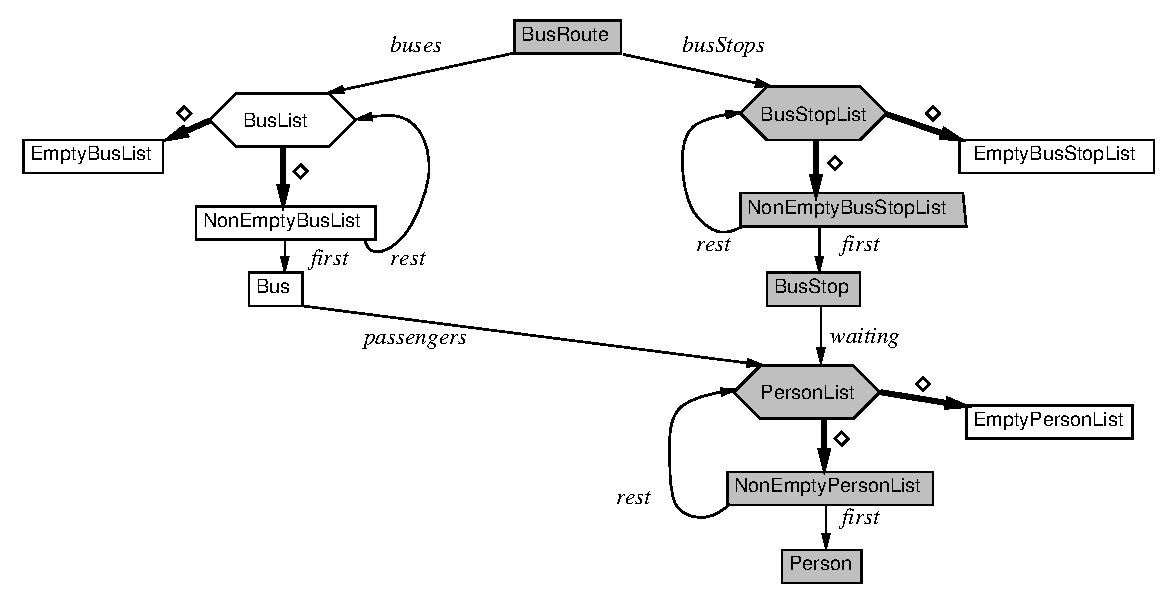
\psfig{file=busstop1.ps,width=\textwidth}}
\caption{\em Bus simulation class graph.  Squares and hexagons denote
classes (concrete and abstract, respectively), regular arrows denote
field reference and are labeled by the field name, and heavy arrows
(labeled with $\diamond$) denote the subclass relation (for the
shading, see text).}
\label{fig-bus1}
\end{figure}

Consider a program simulating bus route management.  For expressing
class graphs, we use the class dictionary graph graphical
representation from the Demeter method~\cite{karl:demeter}.
Alternative notations would be the UML class diagram notation
\cite{rational:UML-LUG} or an XML schema notation~\cite{URL:XMLschema}.
For expressing behavior, we use standard Java and the DJ
library~\cite{OrleansLieberherrReflection01,
adaptive-methods-cacm-2001, URL:demeter}, a Java implementation of the
algorithms in this paper (see Section~\ref{ssec-DJ} for more details
about DJ and our other software).  Consider the class graph depicted
in Figure~\ref{fig-bus1}, which defines a data structure describing a
bus route. A bus route object consists of two lists: a list of bus
objects, each containing a list of passengers; and a list of bus stop
objects, each containing a list of people waiting.  Suppose that as a
part of a simulation, we would like to determine the set of person
objects corresponding to people waiting at any bus stop on a given bus
route.  The group of collaborating classes which is needed for this
task is shaded in Figure~\ref{fig-bus1}. To carry out the simulation,
an object-oriented program would contain a method for each of these
shaded classes.  These methods that are scattered across several
classes would traverse bus route objects.  However, using the
technique of strategies, one can solve the problem in a much more
elegant way, by modularizing the code and keeping it in one place,
rather than scattered through several classes and tangled with other
methods.  We define a strategy graph with nodes {\sf BusRoute}, {\sf
BusStop} and {\sf Person} that are connected by an edge from {\sf
BusRoute} to {\sf BusStop} and an edge from {\sf BusStop} to {\sf
Person}.
% (Note that this is a strategy graph because it is a subgraph
% of the transitive closure of the class graph.)
In our textual syntax, the strategy can be expressed as:
\begin{quote}
\texttt{from BusRoute via BusStop to Person}
\end{quote}

\begin{figure}
\centerline{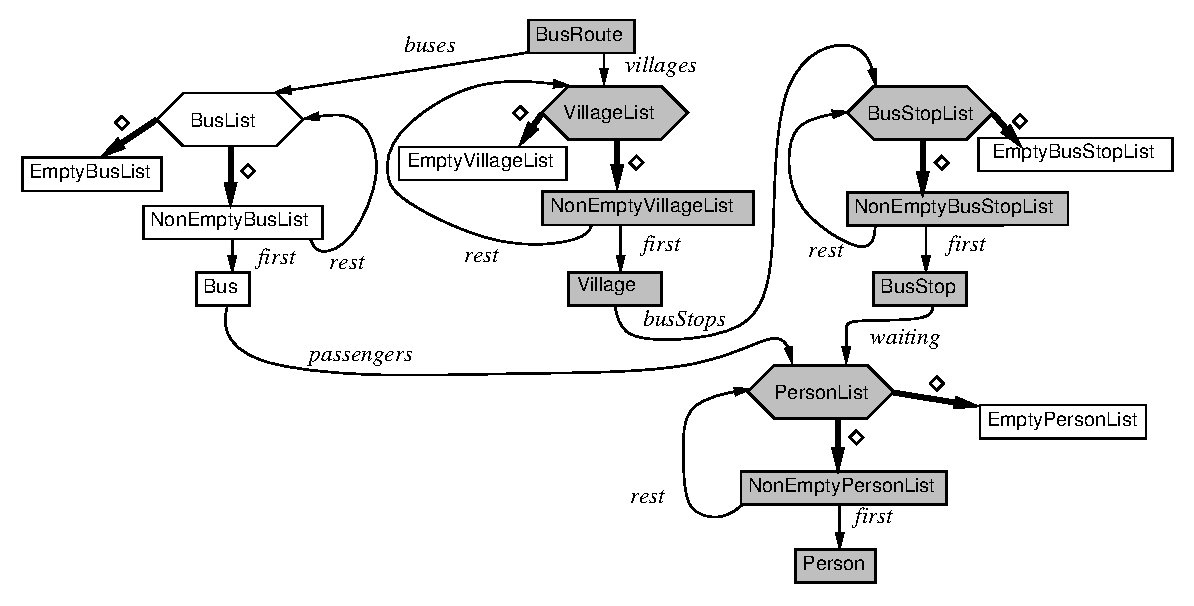
\psfig{file=busstop2.ps,width=\textwidth}}
\caption{\em Evolved bus simulation class graph.}
\label{fig-bus2}
\end{figure}
\noindent

The benefit of strategies is apparent when considering the following
scenario: Suppose that the bus route class has been modified so that
the bus stops are grouped by villages.  The revised class graph is
depicted in Figure~\ref{fig-bus2}. To implement the same requirement of
finding all people waiting for a bus, an object-oriented program must
now contain one method for each of the classes shaded in
Figure~\ref{fig-bus2}, and thus the previous object-oriented
implementation becomes invalid. The traversal strategy,
however, is up-to-date and does not require any rewriting. In
fairness, the revision to the class graph must preserve the class
names referred to in the traversal strategy and the meaning of the
traversal strategy must be correct for the new class graph.  When a
class graph is changed, it is important to check the correctness of
all traversal strategies that depend on that class graph.  Sometimes
it is necessary to refine the strategies to make them correct in the
new class graph, but this is easier than updating all traversal
methods manually~\cite{karl:demeter}.

The actual work on the objects is done by methods on a \emph{visitor}
object: these are methods that can be associated with classes or edges
in the class graph, specifying what to do when the traversal arrives
at an object of a particular type or dereferences a particular field.
Visitor objects are named after the Visitor design
pattern~\cite{gang-of-4} but are much simpler than visitor objects
described by the Visitor design pattern, since none of the scaffolding
is needed---by scaffolding we mean writing an abstract visitor class
that duplicates much information from the class graph.

Strategies effectively filter out the noise in the class graph which
is irrelevant to the implementation of the current task.  For the
class graph in Figure~\ref{fig-bus2}, the above strategy, which
mentions only three classes, replaces methods for ten classes: {\sf
BusRoute, VillageList, NonEmptyVillageList, Village, BusStopList,
NonEmptyBusStopList, BusStop, PersonList, NonEmptyPersonList, Person}.

To show how to program with strategies, we complete the Java program
(using the DJ library) of finding all people waiting at any bus stop
on a particular bus route:
\begin{quote}
\begin{verbatim}
// in class BusRoute:
static ClassGraph cg = new ClassGraph();
static Strategy waiting = new Strategy("from BusRoute via BusStop to Person");
void printWaitingPersons() {
  cg.traverse(this, waiting, new PrintVisitor());
}
\end{verbatim} 
\end{quote}
The program above defines a method called {\sf printWaitingPersons}
for the class {\sf BusRoute}. This method will execute the traversal
specified by the strategy and print the object of class {\sf BusRoute}
using the visitor class {\sf PrintVisitor}.  Note that the definition
of {\sf printWaitingPersons} works without any change for both class
graphs, which is the reason for calling it an {\em adaptive method}
\cite{adaptive-methods-cacm-2001}.

Notice that the adaptive method is expressed in plain Java using the
DJ library of which we use the classes {\sf ClassGraph} and {\sf
Visitor}, the superclass of all visitor classes (such as {\sf
PrintVisitor}).  A {\sf ClassGraph}-object is a graph whose nodes are
classes and whose edges are \emph{is-a} and \emph{has-a} relationships
between classes. Class {\sf ClassGraph} provides methods to create and
maintain a class graph.  The simplest way to create a {\sf
ClassGraph}-object is to call the constructor {\sf ClassGraph()}
without arguments which will create the class graph using Java
reflection by taking all classes in the default package.  A traversal
strategy may be applied to both a {\sf ClassGraph}-object and a
Java object.  From the point of view of a {\sf ClassGraph}-object, a
traversal strategy is a subgraph of the transitive closure of the
{\sf ClassGraph}-object.  When it is applied to a class graph it
selects a subset of the paths in the class graph.  If applied to a
Java object, a traversal strategy defines a subgraph of the
object graph representing the Java object.

In this implementation of adaptive programming with DJ the class graph
and the traversals are computed dynamically.  In other implementations
of adaptive programming (see Section~\ref{ssec-tools}), the traversals
are computed statically.

To show the details of visitors, we write a Java method that counts
(instead of prints) all people waiting at any bus stop on a particular
bus route. Because the traversals for {\sf printWaitingPersons} and
{\sf countWaitingPersons} are identical, we reuse the same {\sf
waiting} traversal strategy.  We also reuse the class graph
{\sf cg}:
\begin{quote}
\begin{verbatim}
  // in class BusRoute:
  int countWaitingPersons() {
    Integer result = (Integer) cg.traverse(this, waiting, new CountVisitor());
    return result.intValue();
  }

class CountVisitor extends Visitor {
  int c;
  public void start() { c = 0; }
  public void before(Person p) { c++; }
  public Object getReturnValue() { return new Integer(c); } 
}
\end{verbatim}
\end{quote}
Class {\sf Visitor} has a simple interface: with the {\sf start}
method we say what needs to be done before the traversal starts.  With
the {\sf getReturnValue} method we express what needs to be returned
when the traversal completes. With a {\sf before} method we express
what needs to be done before we visit an object of a specific class,
specified by the method's argument type.  There are also {\sf after}
and {\sf around} methods; the complete API is documented
in~\cite{URL:demeter}.  The {\sf before}, {\sf after}, and {\sf around}
methods that are defined in a visitor class are invoked using the Java
Reflection API.

\subsection{New Contributions}

The contributions of this paper are three-fold: an extension to the
traversal specification language, a polynomial-time compilation
algorithm for the extended language that is simpler than our earlier
algorithm, and a lower bound result which explains the shortcomings of
the previous algorithms.  More specifically, we allow the underlying
specification of a traversal to have any topology, generalizing the
series-parallel and tree topologies considered previously, and we
allow the use of a name map between nodes in the strategy graph and
those in the class graph. This name map supports the option for
different nodes in the strategy graph to be mapped to the same node in
the class graph.  Section~\ref{sec-comparison} provides a more
detailed comparison of traversal strategies and traversal
specifications.

The generalization of our previous algorithm to a larger class of
graphs was not our primary goal for coming up with a better
algorithm. It happened as a side-effect: as we made the algorithm more
efficient and usable for a larger class of series-parallel graph/class
graph combinations, the resulting algorithm also naturally worked for
any kind of graph.

Our new polynomial-time algorithm presented in Section~\ref{sec-alg}
has the beneficial property that it is simpler and easier to
understand. Our earlier algorithm required an unintuitive check for
the short-cut and zig-zag conditions. Those two conditions had to be
checked to make sure that the traversal is correct. The short-cut and
zig-zag conditions also prohibited many series-parallel graph/class
graph combinations. We notice that this paper is related to two
applications of Polya's inventors paradox\cite{polya:solve-it}:
\begin{enumerate}
\item Although we solve a more general algorithmic problem at the
      programming tool level, the algorithm becomes simpler.
\item The algorithm supports better adaptive programming which is
      about solving problems for more general data structures than the
      one originally given, leading to simpler programs
      (\cite{karl:demeter}, Section 4.1.1).
\end{enumerate}

The compilation algorithm generates code whose running time may be
slightly worse than the running time of the code generated by previous
compilation algorithms (when they apply), since the previous algorithm
generated traversal methods which did not pass arguments at
all. However, this minor penalty in running time is unavoidable if we
want the size of the traversal code to be reasonably bounded: we prove
in Section~\ref{sec-lb} that if no arguments are passed by the
traversal methods, then there are cases where the number of distinct
traversal methods must be exponential in the size of the strategy
specification.

\subsection{Algorithm Overview}
\label{alg-overview}

\newcommand{\first}{\mathit{first}}

For those readers who don't need to understand all the details behind
the algorithms we give a brief overview. Given a strategy $S$ and a
class graph $G$, we need to provide an algorithm that decides which
objects to visit from a node $o$ in an object graph, i.e., we need to
compute $\first(o)$, the set of edges that we need to traverse from
node $o$. The function $\first(o)$ is computed based on answers to
reachability questions in the class graph; it contains all edges that
{\em could} lead (according to the rules of the class graph) to target
objects.  The {\em ``could''} represents our lack of knowledge about
the rest of the object graph~\cite{mitch:karl-2000}.  More precisely,
$\first(o)$ contains all edges $\edge ol{o'}$ such that there exists
an object graph rooted at $o'$ that contains a target object and
that satisfies a fixed set of constraints (expressed by $S$ and $G$).

Our goal is to make the traversal efficient; therefore we don't want
to look ahead in the object graph to decide whether going through an
edge in $\first(o)$ will eventually lead us to a target object.  We
only look ahead in the class graph because it gives us
meta-information about the shape of objects. So $\first(o)$ will
contain all those edges after which, according to the class graph
information, there is still a possibility of reaching a target object.
To quickly answer the reachability questions we compute a new graph,
called a traversal graph, which is basically the product of the two
graphs $S$ and $G$. The traversal graph stores the answers to the
reachability questions that we will ask during the object traversal.

The Traversal Graph Algorithm (TGA) is based on the following idea of
a reduction: For traversal strategies of the form ``{\sf from A to
B}'', the paths defined in the class graph can be represented by a
subgraph of the class graph: Compute all edges reachable from {\sf A}
(called forward edges) and from which {\sf B} can be reached (called
backward edges). This computation is called {\em from-to
computation}. Edges in the intersection of the forward and backward
edges form the graph which represents the traversal.  Any strategy can
be reduced to a from-to computation on a graph that is much larger
than the original class graph. This larger graph, called the traversal
graph, will contain as many copies of the class graph as the traversal
strategy graph has edges.  The size of the traversal graph will be
reduced by a from-to computation.  In other words, the from-to
computation (which can be implemented, e.g., with a forward and a
backward depth-first search) is fundamental to computing the traversal
graph. The size of the traversal graph is a small polynomial in the
size of the class graph and the strategy graph.

The traversal graph is non-deterministic in nature: from a node there
might be two outgoing edges with the same label (leading to different
nodes---there are no parallel edges).  This non-determinism needs to
be handled carefully in order to avoid an exponential blow-up in
algorithm performance.  The Traversal Methods Algorithm (TMA)
traverses an object graph, guided by a traversal graph. To deal with
the non-determinism, we allow multiple tokens simultaneously to be put
on the traversal graph to keep track of the legal traversal
possibilities. As the traversal progresses the number of tokens on the
traversal graph fluctuates. Fortunately, the number of simultaneous
tokens is bounded by the number of edges in the strategy graph.

As suggested by~\cite{gener-comp-j:jens-boaz-karl,Smaragdakis}, these
two algorithms are about computing intersections of sets of paths.
TGA is a variation on an algorithm to compute the cross product of two
automata, while TMA is inspired by the NFA simulation technique
described in~\cite{dragon-nfa-sim}.  The complications are in the
constraint maps, the name maps and the more complex structure of the
graphs: class graphs have two kinds of nodes and two kinds of edges.


\subsection{Paper Organization}

The remainder of this paper is organized as follows.  In Section
\ref{sec-prel} we introduce the basic concepts, terminology and
notation we use throughout the paper.  In Section~\ref{sec-traversals}
we give a definition for the concept of traversals, based on
\cite{gener-comp-j:jens-boaz-karl}.  In Section~\ref{sec-strategy} we
define the new concept of strategies.  In Section~\ref{sec-alg} we
specify and analyze the algorithm which translates strategies into
traversal code.  In Section~\ref{sec-lb} we prove a lower bound for
traversal methods that do not pass arguments.  In Section
\ref{sec-notes} we comment about some practical aspects of the
implementation of the strategies approach.  In Section
\ref{sec-related} we survey related work.  In Section
\ref{sec-comparison} we compare strategies with the earlier approach
of traversal specifications.  In Section~\ref{sec-appls-trav-strats}
we describe some applications of strategies.  In Section
\ref{sec-experience} we describe our experiences using strategies and
present some empirical evidence of how they are used.  We give a few
concluding thoughts in Section~\ref{sec-conc}.

\section{Preliminaries}
\label{sec-prel}
%%%%%%%%%%%%%%%%%%%%%%%%%
In this section we formally define the basic concepts, terminology and
notation we use throughout this paper. All notions in this section are
standard, with the exception of Subsection~\ref{ssec-assumptions}.

\subsection{Graphs and paths}
%%%%%%%%%%%%%%%%%%%%%%%%%%%%%%%%%%%%%%%%%%%%
A directed graph is a pair $(V,E)$ where $V$ is a set of {\em nodes},
and $E\subseteq V\times V$ is a set of {\em edges}.  A directed
labeled graph is a triple $G=(V,E,L)$ where $V$ is a set of {\em
nodes}, $L$ is a set of {\em labels}, and $E\subseteq V \times L
\times V$ is a set of {\em edges}.  If $e=(u,l,v) \in E$, then $u$ is
the {\em source} of $e$, $l$ is the {\em label} of $e$, and $v$ is the
{\em target} of $e$.  We denote an edge $(u,l,v)$ by $\edge u l v$.

Given a directed labeled graph $G=(V,E,L)$, a {\em node-path} is a
sequence $p=\Seq{v_0v_1\ldots v_n}$, where $v_i\in V$ for $0\le i\le
n$, and $\edge{v_{i-1}}{l_i}{v_i}\in E$ for some $l_i\in L$ for all
$0<i\le n$.  Similarly, a {\em path\/} is a sequence
$\Seq{v_0l_1v_1l_2\ldots l_nv_n}$ where $\Seq{v_0\ldots v_n}$ is a
node-path, and $\edge {v_{i-1}}{l_{i}}{v_{i}}\in E$ for all $0< i\le
n$.  Unlabeled graphs have only node-paths.  Paths of the form
$\Seq{v_0}$ are called {\em trivial.}  The first node of a path (or a
node-path) $p$ is called the {\em source} of $p$, and the last node in
$p$ is called the {\em target} of $p$, denoted $\Source(p)$ and
$\Target(p)$, respectively.  The elements other than the source and
the target of a path (nodes for a node-path, nodes and edges for a
path) are the {\em interior} of the path.  For a graph $G$, nodes
$u,v$, and sets of nodes $U,V$, we define $P_G(u,v)$ to be the set of
all paths in $G$ with source $u$ and target $v$ and $P_G(U,V)$ to be
the set of all paths in $G$ with source in $U$ and with target in $V$.

If $p_1 = \Seq{v_0 \ldots l_i v_i}$ and $p_2 = \Seq{v_{i}
l_{i+1}\ldots v_n}$ are paths with the target of $p_1$ identical to
the source of $p_2$, we define the concatenation $p_1 \cdot p_2 =
\Seq{v_0 \ldots v_{i-1}l_i v_{i}l_{i+1}v_{i+1} \ldots v_n}$.  Notice
that $p_1 \cdot p_2$ contains only one copy of the meeting point
$v_i$. Concatenation of node paths is defined similarly.  Let $P_1$
and $P_2$ be sets of paths such that for some node $v$,
$\Target(p_1)=v$ for all $p_1\in P_1$, and $\Source(p_2)=v$ for all
$p_2\in P_2$.  Then we define
$$
P_1 \cdot P_2 = \Set{ p_1 \cdot p_2\mid p_1 \in P_1\mbox{ and }p_2 \in P_2}~.
$$

\subsection{Class graphs and object graphs}
%%%%%%%%%%%%%%%%%%%%%%%%%%%%%%%%%%%%
In this paper we will be interested in special kinds of graphs, called
class graphs and object graphs, defined as follows.

Fix a finite set $\cC$ of {\em class names}.  Each class name is
either {\em abstract} or {\em concrete}.  Fix a finite set $\cL$ of
{\em field names}.  We sometimes call field names {\em labels}.  We
assume the existence of two distinguished symbols: $\This\in\cL$ and
$\diamond\notin\cL$.  Class graphs model the class structure of
object-oriented programs.  Formally, {\em class graphs} are graphs
$G=(V,E,L)$ such that
\begin{itemize}
\item $V\subseteq\cC$, i.e., the nodes are class names.
\item $L\subseteq\cL\cup\Set{\diamond}$, i.e., edges are labeled by
      field names or ``$\diamond$''. Edges labeled by a field name are
      called {\em reference} edges, and edges
      labeled by $\diamond$ are called {\em subclass} edges.
\item For each $v\in V$, the field names of all edges going out from
      $v$ are distinct (but there may be many edges labeled by
      $\diamond$ going out from $v$).
\item For each $v\in V$ such that $v$ is concrete, $\edge v\This v\in E$.
\item The set of subclass edges is acyclic.
\end{itemize}
%
We shall use the (reflexive) notion of a {\em superclass\/}: given a
class graph $G=(V,E,L)$, we say that $v\in V$ is a superclass of $u\in
V$ if there is a (possibly empty) path of subclass edges from $v$ to
$u$. The collection of all super-classes of a class $v$ is called the
{\em ancestry} of $v$.  Multiple inheritance conflicts are disallowed:
we require that the following condition holds true.
\begin{quote}
{\bf Single Inheritance Condition:} For all nodes $v$, if $v$ has two
superclasses $u$ and $w$ with outgoing edges labeled by the same
label, then either $u$ is in the ancestry of $w$ or $w$ is in the
ancestry of $u$.
\end{quote}
The set of {\em induced references} of a given class $v$ is the set of
all reference edges going out from its ancestry, with the usual
overriding rule: for each label $l$ used in edges going out from the
ancestry of $v$, only the edge labeled $l$ closest to $v$ is in the
induced references of $v$. The notion of ``closest'' is well defined
by the Single Inheritance Condition above.  Note that since a class is
a superclass of itself, the induced edges include both the direct
references and the inherited references.

Next, we define {\em object graphs}, which model the instantiations of
class graphs.  An object graph is a labeled directed graph
$\Omega=(V',E',L')$, where nodes are called {\em objects}, and
$L'\subseteq\cL$.  An object graph $\Omega=(V',E',L')$ is an {\em
instance} of a class graph $G=(V,E,L)$ under a given function $\Class$
mapping objects to classes, if the following conditions are satisfied.
\begin{itemize}
\item For all objects $o\in V'$, $\Class(o)$ is concrete.
\item For each object $o\in V'$, the labels of edges going out from
      $o$ is exactly the set of labels of the induced references of
      $\Class(o)$. (In particular, this means that the edges going out
      from $o$ have distinct labels.)
\item For each edge $\edge o l {o'}\in E'$, $\Class(o)$ has an induced
      reference edge $\edge v l u$ such that $v$ is a superclass of
      $\Class(o)$ and $u$  is a superclass of $\Class(o')$.
\end{itemize}
For the greater part of this paper, we shall assume that object graphs
are acyclic. We discuss an extension to cyclic object graphs in
Section~\ref{sec-ext}.

\subsection{Non-standard notions}
\label{ssec-assumptions}
%%%%%%%%%%%%%%%%%%%%%%%%%%%%%%%%%%%%%

In this paper, we assume that class graphs are {\em simple}, formally
defined as follows.

\begin{definition}
\label{def-simple}
A class graph $G=(V,E,L)$ is {\sf simple} if 
\begin{enumerate}
\item for all edges $\edge u l v \in E$, we have that $l=\diamond$ if
      and only if $u$ is abstract, and
\item for all edges $\edge u\diamond v \in E$, we have that $v$ is concrete.
\end{enumerate}
\end{definition}
%
The first requirement says that all edges going out from abstract
classes are subclass edges and all edges going out from concrete
classes are reference edges.  This property is called {\em flatness}.
Flatness helps us map paths in a class graph $G$ to paths in an object
graph which is an instance of $G$. The second requirement says that
all subclass edges are coming into concrete classes; this helps us
find all subclasses of a given class quickly.  Note that no generality
is lost by the assumption that class graphs are simple, as the
following proposition asserts.
%
\begin{proposition}
\label{prop-simple}
Let $G=(V,E,L)$ be an arbitrary class graph. Then there exists a
simple class graph $\Simple(G)=(V',E',L)$ such that an object graph
$\Omega$ is an instance of $G$ if and only if $\Omega$ is an instance
of $\Simple(G)$. Moreover, $|V'|=O(|V|)$ and $|E'|=O(|E|^2)$.
\end{proposition}
The $\Simple$ transformation is outlined in Appendix~\ref{sec-simpleten}.
Note that the output of our compilation algorithm is a set of methods
on an arbitrary class graph, i.e.~it need not be simple.  An existing
class structure does not need to be modified to be used with our
algorithm; it is only the graph representation of the class structure
that may need to be pre-processed by the $\Simple$ transformation.

Define a {\em concrete path} to be an alternating sequence of concrete
class names and labels (excluding $\diamond$).  We shall map paths in
class graphs to concrete paths by omitting abstract classes and
subclass edges.  We refer to this mapping as the {\em natural
correspondence}, and denote it by $X(p)$, where $p$ is a path in a
class graph $G$ and $X(p)$ is the corresponding concrete path.
Similarly, we denote the concrete path resulting from taking the
sequence of class names and edge labels in an object graph path $p'$
by $Y(p')$, and (overloading the term) we call this mapping also a
{\em natural correspondence}.  The motivation for these definitions is
that if $p$ is a path in a class graph $G$, then there is some object
graph $\Omega$ which is an instance of $G$, and a path $p'$ in
$\Omega$, such that $X(p)=Y(p')$.

For a class graph path set $P$, define $X(P)\DEF\Set{X(p)\mid p\in P}$.

\section{Definition of traversals}
\label{sec-traversals}
%%%%%%%%%%%%%%%%%
We now arrive at the central topic of this paper: traversals of object
graphs.  Informally, a traversal is a (possibly infinite) set of
concrete paths; when used in conjunction with an object graph, it
results in a sequence of objects, called the {\em traversal
history}. The traversal history is a depth-first traversal of the
object graph along object paths agreeing with the given concrete path
set.  To make the traversal useful, each object has a special {\em
visit} method attached to it; when an object is added to the traversal
history, this method is invoked.  (A more comprehensive discussion of
the Visitor design pattern and visitor methods can be found in
\cite{gang-of-4,spl:context-conf,seiter:ieee-se-98}.)

But first, we define traversals formally.  The definition here is
adapted from the ``simplified semantics'' from
\cite{gener-comp-j:jens-boaz-karl}.  We use a few technical notions.
For a set of sequences $R\subseteq\Sigma^*$ for an alphabet $\Sigma$,
define
\(
\First(R) &=& \{x\in\Sigma \mid \exists\alpha.(x\alpha\in R)\} \\
\Chop(R,x)&=& \{\alpha \mid x\alpha\in R\mbox{ for some }x\in\Sigma\}\ .
\)
Intuitively, $\First(R)$ is the set of all first elements of $R$, and
$\Chop(R,x)$ is the set of all ``tails'' of sequences of $R$ that
start with $x$ (where a tail of a sequence is the whole sequence
except its first element).

In the definition below, we assume that there exists a total order
$\prec$ on the set of field names $\cL$ (this assumption may be
weakened somewhat). We first give the formal definition, then explain
it in words.

\begin{definition}[from~\cite{gener-comp-j:jens-boaz-karl}]
\label{def-traversal}
Fix a class graph $G$.  If $\Omega$ is an acyclic object graph which
is an instance of $G$, $o$ an object in $\Omega$, $R$ a set of
concrete paths corresponding to paths of $G$, and $H$ a sequence of
objects, then the judgment $$\Omega \vdash_s o:R \rhd H$$ means that
when traversing the object graph $\Omega$ starting with $o$, and
guided by the concrete path set $R$, then $H$ is the {\sf traversal
history}.%
\footnote{The label $s$ of the turnstile indicates ``semantics.''}
This judgment holds when it is derivable using the following rules:
\begin{equation}
\label{eq-traversal-empty}
\irule{}
      {\Omega \vdash_s o: R \rhd \epsilon}
   ~~~~~~
      \parbox{3in}{
       if $\Chop(R,\Class(o))=\emptyset$,}
\end{equation}
where $\epsilon$ denotes the empty history, and
\begin{equation}
\label{eq-traversal-recursive}
\irule{\Omega \vdash_s o_i: \Chop(\Chop(R,\Class(o)),l_i) \rhd H_i
       \air \forall i \in 1..n}
      {\Omega \vdash_s o: R \rhd o \cdot H_1  \cdot ... \cdot H_n}
   ~~~~~~
      \parbox{3in}{
       if $\First(\Chop(R,\Class(o))) = \{l_i \mid i \in 1..n\}$, \\
                   $\edge o {l_i} {o_i} \mbox{ is in } \Omega,
                   i \in 1..n$, and \\
                   $l_j \prec l_k \mbox{ for } 1 \leq j < k \leq n$.}
\end{equation}
\end{definition}
%
In other words, a traversal of an object graph $\Omega$ starting with
an object $o$ guided by a path set $R$, is done as follows.  First,
the first elements of the sequences of $R$ are compared to
$\Class(o)$: sequences beginning with another element are immediately
thrown out of consideration. If the remaining path set is not empty,
then $o$ becomes the first element of the history; it is followed by
the histories resulting from starting a traversal from each descendent
of $o$, guided by the remainder of the path set after ``peeling off''
the first two elements (corresponding to $o$ and the edge going out to
the descendent). Intuitively, this procedure is depth-first search on
$\Omega$ with $R$ used to determine how to prune the search.  Please
note that concatenation of traversal histories does not use the same
definition as concatenation of paths; it is the usual concatenation of
sequences.

\paragraph{Remarks.}
Note that the guarantee made by a traversal guided by a path set $R$
is the following: A path $p$ in the object graph is followed so long
as there is a path $q\in R$ such that $q$ has a prefix which is
equal to the current prefix of $p$ (taking the $\Class(o)$ instead of
$o$ in $p$). In other words, the decision whether the traversal takes
a certain branch in the object graph depends only on the portion of
the graph visited so far and on the current branch, and not on the
links further ahead. This means, for example, that even if all paths
in $R$ end with the same class $A$, some of the traversal paths may
end with a node $o$ with $\Class(o)\ne A$ just because the path to $o$
is a prefix of a path in $R$.  This relaxation is necessary to enable
efficient implementation of traversals by looking only ahead in the
class graph and not in the object graph as discussed earlier.


\section{Strategies: Specification of traversals}
\label{sec-strategy}
%%%%%%%%%%%%%%%%%%%%
In this section we define strategies, which are a graph-based language
for expressing traversals. In Section~\ref{ssec-simple-strategy} we
give a basic definition of strategies and explain how strategies
express traversals.  Then, in Section~\ref{ssec-full-strategy}, we
give the full definition of strategies using the additional concept of
a constraint map. This extended notion is the one we shall be using in
the remainder of the paper. In Section~\ref{ssec-strategies-ext}, we
discuss a few possible additional refinements of the concept of
strategies.

\subsection{Strategies}
\label{ssec-simple-strategy}
%%%%%%%%%%%%%%%%%%%%%%%%%%%%%%
Traversals are defined in terms of sets of concrete paths. Strategies
select class graph paths and then derive concrete paths by applying
the natural correspondence.  Intuitively, a strategy selects class
graph paths by specifying a high-level topology which spans all paths
in the selected set.  Formally, strategies are defined as follows.

\begin{definition}
A {\sf strategy} $\cS$ is a triple $\cS=(S,s,t)$, where $S=(C,D)$ is a
directed unlabeled graph called the {\sf strategy graph}, where $C$ is
the set of {\sf strategy graph nodes} and $D$ is the set of {\sf
strategy graph edges}, and $s,t\in C$ are the {\sf source} and {\sf
target} of $\cS$, respectively.
\end{definition}
%
The connection between strategies and class graphs is done by a name map,
defined as follows.

\begin{definition}
Let $S=(C,D)$  be a  strategy graph and let $G=(V,E,L)$ be a class
graph. A {\sf name map} for $S$ and $G$ is a function
$\cN:C\rightarrow V$. If $p$ is a sequence of strategy graph nodes,
then $\cN(p)$ is the sequence of class nodes obtained by applying $\cN$
to each element of $p$.
\end{definition}

The basic idea of strategies is that under a name map, a path in the
strategy graph is an abstraction of a set of paths in the class
graph. This is done by viewing each strategy graph edge $\edge a{}b$
as representing the set of paths in the class graph starting with node
$\cN(a)$ and ending at node $\cN(b)$.  This representation naturally
extends to paths in the strategy graph: A path in the strategy graph
represents a set of paths in the class graph obtained by concatenating
the sets of class graph paths obtained from each strategy graph edge.

We now make this intuition formal using the concept of path expansion,
defined as follows.

\begin{definition}
Given a nontrivial sequence $p$, a sequence is called an {\sf expansion} of $p$
if it can be obtained by inserting one or more elements between the elements of
$p$.  The only expansion of a trivial sequence is itself.
\end{definition}
%
Note that if $p'$ is a path which is an expansion of another path $p$
(possibly in another graph), then
$\Source(p)=\Source(p')$ and $\Target(p)=\Target(p')$.

We now formally define the basic way strategies express paths in
object graphs.  Recall that $P_G(s,t)$ denotes that set of all paths
in $G$ starting at $s$ and ending at $t$ and $X$ is the natural
correspondence mapping class graph paths to concrete paths.

\begin{definition}
Let $\cS=(S,s,t)$ be a strategy, let $G=(V,E,L)$ be a class graph, and
let $\cN$ be a name map for $\cS$ and $G$. Then
$$
\cS[G,\cN]=\Bigl\{
X(p')\mid p'\in P_G(\cN(s),\cN(t))\mbox{ and }
 \exists p\in P_S(s,t)\mbox{ such that }p'\mbox{ is an expansion of }\cN(p)
\Bigr\}~.
$$
\end{definition}
%
Note that $\cS[G,\cN]$ is a set of concrete paths: intuitively, first
a set of class graph paths is selected, and then the natural
correspondence is applied to obtain concrete paths.  These concrete
paths can be used (playing the role of ``$R$'') in Definition
\ref{def-traversal}.

\subsection{Using a constraint map}
\label{ssec-full-strategy}
%%%%%%%%%%%%%%%%%%%%%%%%%%%%%%%%
Strategies impose positive constraints on paths, in the sense that
they specify which nodes must be traversed in which order. It turns
out that it is quite useful to also have negative constraints: what
nodes and edges cannot be used between the specified milestones.  We
formalize this idea with the concepts of element predicates and
constraint maps.

\begin{definition}
Given a class graph $G=(V,E,L)$, an {\sf element predicate} $EP$ for
$G$ is a predicate over $V\cup E$. Given a strategy graph $S$, a
function $\cB$ mapping each edge of $S$ to an element predicate for
$G$ is called a {\sf constraint map} for $S$ and $G$.
\end{definition}
%
(Of course, some predicate specification languages may be very hard to
compute. For computational complexity purposes, we assume that there
exists a parameter, denoted $\tau$, such that given an element of $G$,
determining whether it satisfies an element predicate can be computed
in no more than $\tau$ time units.)

The constraint map is used to specify, for each edge in the strategy
graph, which elements of the class graph may be used in the traversal
corresponding to that edge.  Formally, we have the following
definition.

\begin{definition}
\label{def-sat}
Let $S$ be a strategy graph, let $G$ be a class graph, let $\cN$ be a
name map for $S$ and $G$, and let $\cB$ be a constraint map for $S$
and $G$.  Given a strategy graph node path $p=\Seq{a_0a_1\ldots a_n}$, we
say that a class graph path $p'$ is a {\sf satisfying expansion} of
$p$ with respect to $\cB$ under $\cN$ if there exist nontrivial paths
$p_1,\ldots,p_n$ such that $p'=\Seq{\cN(a_0)}\cdot p_1\cdot p_2\cdots
p_n$ and:
\begin{enumerate}
\item
\label{cond-st}
For all $1\le i\le n$, $\Source(p_i)=\cN(a_{i-1})$ and
$\Target(p_i)=\cN(a_i)$.
\item
\label{cond-sat}
For all $1\le i\le n$, the interior elements of $p_i$ satisfy the
element predicate $\cB(\edge{a_{i-1}}{}{a_i})$.
\end{enumerate}
If $n = 0$, i.e., $p$ is a trivial path $\Seq{a_0}$, then its only
satisfying expansion is $\Seq{\cN(a_0)}$.
\end{definition}
Note that there may be many ways to decompose a path in accordance
with Condition~\ref{cond-st} in the definition above; a path $p'$ is a
satisfying expansion of a path $p$ if for one of these decompositions,
Condition~\ref{cond-sat} holds as well.%
\footnote{
Other definitions are possible, for example to require that a subpath
ends when its target node is reached.  We have found the
non-deterministic definition above to be the most useful.  Constraint
maps can be used to reduce or eliminate the non-determinism.
}
Note also that the element constraints are never applied to the ends
of the sub-paths.

One consequence of our definition is that every edge in a strategy
graph path corresponds to one or more class graph edges in a
satisfying expansion: if $\cN(a_{i-1})=\cN(a_i)$, the path $p_i$ may
not be the trivial path $\Seq{\cN(a_i)}$.  A further consequence is
that every class graph edge in a satisfying expansion satisfies at
least one element predicate in the constraint map.

Using the constraint map, we now define a more elaborate way in which
a strategy expresses paths in object graphs.

\begin{definition}
\label{def-strategy-paths}
Let $\cS=(S,s,t)$ be a strategy, let $G=(V,E,L)$ be a class graph, let
$\cN$ be a name map for $S$ and $G$, and let $\cB$ be a constraint map
for $S$ and $G$.  Then $\cS[G,\cN,\cB]$ is the set of concrete paths
defined by
$$
\begin{array}{ll}
\cS[G,\cN,\cB]=\Bigl\{X(p')\mid&
p'\in P_G(\cN(s),\cN(t))\mbox{ and }\\
&\exists p\in P_S(s,t)\mbox{ such that $p'$ is a satisfying expansion of $p$
w.r.t. $\cB$}\;
\Bigr\}~.
\end{array}
$$
\end{definition}
%
Note that $\cS[G,\cN]=\cS[G,\cN,\cB_\True]$ for the constraint map
$B_\True$ which maps all strategy graph edges to the trivial element
predicate that is always $\True$.

\subsection{Remarks}
\label{ssec-strategies-ext}
%%%%%%%%%%%%%%%%%%%%%%%%%%%%%%%%%%%%
\paragraph{Encapsulated strategies.}
The way strategies are presented above, a constraint map can be
specified only when the class graph is given, as the element
predicates are expressed in terms of class graph nodes and edges. An
important design consideration, however, is to encapsulate the
constraint map with the strategy and use the name map as the only
interface to the class graph; we call this approach ``encapsulated
strategies.'' The advantage of encapsulated strategies is that they
allow one to have a clean interface between the strategy and the class
graph, captured completely by the name map.

We only outline the details of the concept here, since it is not
central to the algorithmic issues we focus on in the remainder of this
paper.  The idea is that instead of letting the element predicates
range over the (yet unspecified) class graph, they range over
variables called {\em symbolic names}.  Binding to actual class graph
elements is done only later, when the name map is introduced.
Technically, we have an additional level of indirection in the
encapsulated strategy: instead of explicit references to the class
graph elements in the constraint map, the element predicates are
predicates over {\em symbolic nodes} and {\em symbolic edges.}  These
are denoted using a set $\cM$ of strings, which are used as
place-holders for class names and labels (symbolic edges are
constructed from a pair of symbolic node names and a symbolic label).
More formally, an {\em encapsulated strategy} is a tuple
$\cE=(\cS,\cM,\cB')$, where $\cS$ is a strategy, $\cM$ is a set of
symbolic names, and $\cB'$ is a function mapping edges of the strategy
graph to predicates over the symbolic elements.  To support
encapsulated strategies, the name map is extended to map also symbolic
names to actual class names and label names in the class graph.

\paragraph{Wildcard notation in predicate specification.}
We left the issue of how to specify the predicates open. One naive way
of doing it is to enumerate all elements to be used, or alternatively
to enumerate all elements to be excluded (cf.\ ``only-through'' and
``bypassing'' clauses presented in Section~\ref{ssec-syntax}).  More
expressive power is given by allowing wildcard symbols to be used in
the predicate specification. For example, an element predicate may be
$\False$ for all elements of the form $\edge * l *$, which means that
no edges labeled $l$ can be traversed.  The unique feature of this
notation is that it allows the programmer to refer to elements whose
identity is not necessarily known at predicate-specification
time. Even when using encapsulated strategies as above, the programmer
can only refer to symbolic names, which are later mapped to only a
subset of the elements of the actual class graph, while the wildcard
notation is implicitly mapped to all elements in the class graph as
appropriate.

There is a difference between the strategies used by the algorithm, on
the one hand, and the data structures available in our implementation
(described in Section~\ref{sec-notes}).  In the former, strategy graph
edges are general, with a restriction only on the cost of verifying
the governing condition per vertex and per edge.  In the latter, only
a small set of predefined predicates are used (bypassing,
only-through).  The reason for this difference is that we wanted the
abstract model to be easy to express and it turned out that a more
general formulation is easier to express.  The general model can
easily handle the particular edge predicates actually in use in the
implementation.  For the current applications the expressive power of
the model used by our implementation is sufficient.  Indeed, when the
class graph is known, all strategies can be simulated by single edge
strategies using bypassing clauses bypassing sufficiently many nodes
and edges in the class graph.

\paragraph{Cyclic graphs.}
Strategy graphs may be cyclic and so may class graphs and object
graphs. However for the purpose of dealing with traversals, it is
sufficient to consider object trees. Non-object trees need to be
addressed by appropriate visitors.  See Section~\ref{sec-ext} for more
discussion.

\section{Compilation algorithm}
\label{sec-alg}
%%%%%%%%%%%%%%%%%%%%%%%%%%%%%%%
In this section we show how to implement traversal strategies 
efficiently by compiling them into  executable programs.
Formally, the compilation problem is defined as follows.

\begin{description}
\item[Input:] A strategy $\cS=(S,s,t)$, a simple class graph
$G=(V,E,L)$, a name map $\cN$ for $S$ and $G$, and a constraint map
$\cB$ for $S$ and $G$.
\item[Output:] A set of methods such that for any object graph
$\Omega$, invoking the traversal method at an object $o$ in $\Omega$
yields a traversal history $H$ satisfying the judgment
$\Omega\vdash_{s}o:\cS[G,\cN,\cB]\rhd H$.
\end{description}
Recall that $\cS[G,\cN,\cB]$ is a path set which can guide traversals
of object graphs directly. Our compilation consists of two
algorithms. For an overview of the algorithms see Section
\ref{alg-overview}.

\begin{enumerate}

\item We first invoke an algorithm (called TGA below) which uses
$\cS$, $G$, $\cN$, and $\cB$ to construct a graph which expresses the
traversal $\cS[G,\cN,\cB]$ in a more convenient way; we call this
graph the {\em traversal graph}, and denote it by
$\TG(\cS,G,\cN,\cB)$.

\item We then generate traversal methods that employ another algorithm
      (called TMA below), which uses $\TG(\cS,G,\cN,\cB)$---the result
      of TGA---at runtime.
\end{enumerate}
The remainder of this section is organized as follows.  In Section
\ref{ssec-TG} we describe TGA.  In Section~\ref{ssec-TM} we
describe TMA.  In Section~\ref{ssec-analysis} we analyze the
computational complexity of the algorithms.  We conclude this section
with numerous extensions and variants for the basic algorithm, listed
in Section~\ref{sec-ext}.

\subsection{The traversal graph}
\label{ssec-TG}
%%%%%%%%%%%%%%%%%%%%%%%%%%%%%%%%%%%%%%%%
In this section we explain how the {\em traversal graph} is computed,
based on a strategy $\cS=(S,s,t)$, a simple class graph $G=(V,E,L)$, a
name map $\cN$ for $S$ and $G$, and a constraint map $\cB$ for $S$ and
$G$.  The traversal graph, denoted $\TG(\cS,G,\cN,\cB)$, is created by
a series of transformations based on the class graph, the strategy,
the name map, and the constraint map. The basic idea is to replace
each strategy graph edge by a copy of the class graph appropriately
pruned down to elements that satisfy the edge's element predicate.

The reader may follow a running example presented in
Figure~\ref{fig-comp} (DJ code for the example is given in
Section~\ref{sec-notes}).
\begin{figure}
\centerline{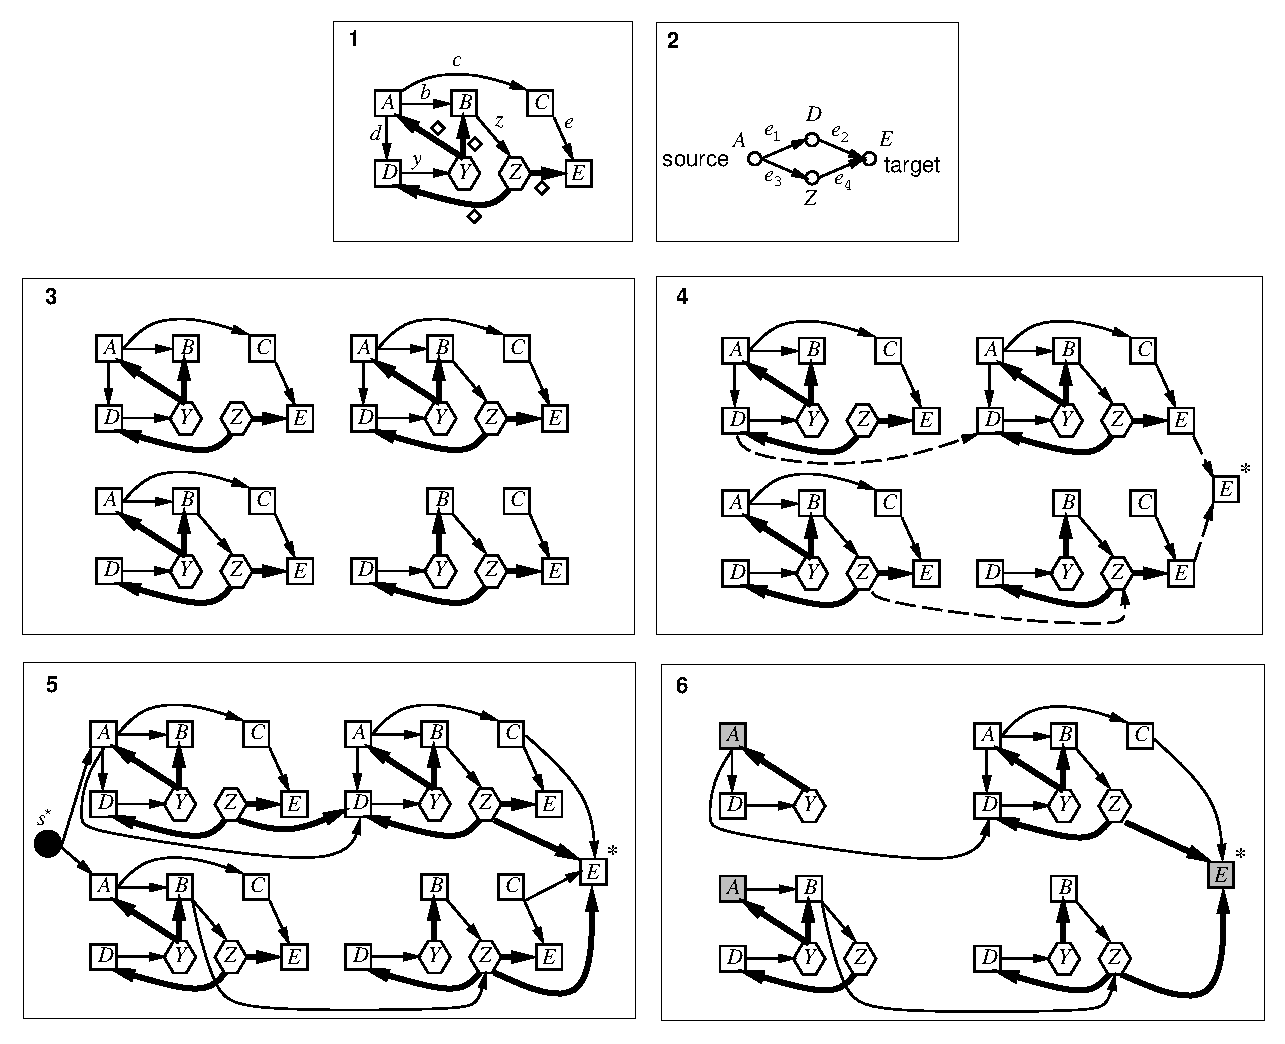
\psfig{file=comp.ps,height=6in}}
\caption{\em An example of traversal graph computation.  {\sf 1}: the
input class graph. Edge labels are omitted from subsequent graphs.
{\sf 2}: The input strategy (the name map is indicated).  In this
example, the constraint map is as follows: $\cB(e_1)(\edge B z
Z)=\False$ and $\cB(e_1)(x)=\True$ for all $x\ne\edge B z Z$;
$\cB(e_2)(x)=\True$ for all $x$; $\cB(e_3)(\edge A d D)=\False$ and
$\cB(e_3)(x)=\True$ for all $x\ne\edge A d D$; and
$\cB(e_4)(x)=\False$ if $x=A$ or if $x$ is an edge incident to $A$,
and $\cB(e_4)(x)=\True$ otherwise.  {\sf 3}: $G'$ after
Steps~\protect\ref{step-replicate} and \protect\ref{step-predicate}.
{\sf 4}: $G'$ after Steps~\protect\ref{sstep-inter}
and~\protect\ref{sstep-target}.  Intercopy edges are dashed.  {\sf 5}:
$G'$ after Steps~\ref{sstep-add},~\ref{sstep-remove},
and~\protect\ref{step-source}.  {\sf 6}: The final traversal graph, as
returned in Step~\protect\ref{step-return}. The shaded $A$ nodes are
the start set $T_s$, and the shaded node $E^*$ is the finish set
$T_f$.}
\label{fig-comp}
\end{figure}

\vbox{\vspace*{3mm}\hrule width \linewidth height 0.5pt\vspace*{-1.5mm}}
\noindent
{\bf Traversal Graph Algorithm (TGA):} Let the strategy graph be
$S=(C,D)$, and let the strategy graph edges be
$D=\Set{e_1,e_2,\ldots,e_k}$.
\begin{enumerate}
\item
\label{step-replicate}
Create a graph $G'=(V',E')$ by taking $k$ copies of $G$, one for each
strategy graph edge.  Denote the $i$th copy as $G^i=(V^i,E^i)$. We
will use the correspondence between each strategy graph edge $e_i$ and
$G^i$.  The nodes in $V^i$ and edges in $E^i$ will be denoted with a
superscript $i$, as in $v^i,e^i$ etc. Each class graph node $v$
corresponds to $k$ nodes in $V'$, denoted $v^1,\ldots,v^k$.  We extend
the $\Class$ mapping to apply to the nodes of $G'$ by setting
$\Class(v^i)\DEF v$, where $v^i\in V'$ and $v\in V$.

\item
\label{step-predicate}
For each strategy graph edge $e_{i}=\edge a{}b$: Let $\cN(a)=u$ and
$\cN(b)=v$. Remove from $G^i$ the elements which do not satisfy
$\cB(e_i)$. More precisely, set
$$
\begin{array}{lll}
V^i&\gets&\Set{u^i,v^i}\cup\Set{w^i\mid\cB(e_i)(w)=\True}~\mbox{, and}\\
E^i&\gets&\Set{\edge{u^i}{l}{v^i}\mid\cB(e_i)(\edge{u}{l}{v})=\True}\cup\\
&&\Set{\edge{u^i}{l}{y^i}\mid\cB(e_i)(\edge{u}{l}{y})=
\cB(e_i)(y)=\True}\cup\\
&&\Set{\edge{w^i}{l}{v^i}\mid\cB(e_i)(\edge{w}{l}{v})=
\cB(e_i)(w)=\True}\cup\\
&&\Set{\edge{w^i}{l}{y^i}\mid\cB(e_i)(\edge{w}{l}{y})=
\cB(e_i)(w)=\cB(e_i)(y)=\True}~.
\end{array}
$$

\item
\label{step-divert}
\begin{enumerate}
\item
\label{sstep-inter}
For each strategy graph node $a\in C$: Let
$I=\Set{e_{i_1},\ldots,e_{i_n}}$ be the set of strategy graph edges
coming into $a$, and let $O=\Set{e_{o_1},\ldots,e_{o_m}}$ be the set
of strategy graph edges going out from $a$.  Let $\cN(a)=v\in V$.  Add
to $G'$ $n\cdot m$ edges $\edge{v^{i_j}}{}{v^{o_l}}$ for $j=1,\ldots,
n$ and $l=1,\ldots,m$. Call these edges {\em intercopy edges.}
\item
\label{sstep-target}
Add to $G'$ a node $\cN(t)^*$ and, for each edge $e_i$ coming into the
target node $t$ in $S$, an intercopy edge $\edge{\cN(t)^i}{}{\cN(t)^*}$.
\item
\label{sstep-add}
For each node $v^i$ in $G'$ with an outgoing intercopy edge: Add to
$G'$ edges $\edge{u^i}l{v^j}$ for all $u^i$ and $v^j$ such that
$\edge{u^i}{l}{v^i}\in E^i$ and $\edge{v^i}{}{v^j}$ is an intercopy
edge.
\item
\label{sstep-remove}
Remove all the intercopy edges added in Steps~\ref{sstep-inter} and
\ref{sstep-target}.
\end{enumerate}

\item
\label{step-source}
Add to $G'$ a node $s^*$ and, for each edge $e_i$ going out from the
source node $s$ in $S$, an edge $\edge{s^*}{}{\cN(s)^i}$.
If $s=t$, add to $G'$ an edge $\edge{s^*}{}{\cN(t)^*}$.

\item
\label{step-cleanup}
Mark all nodes and edges in $G'$ which are both reachable from $s^*$
and from which $\cN(t)^*$ is reachable, and remove unmarked nodes and edges
from $G'$.  Call the resulting graph $G''=(V'',E'')$.

\item
\label{step-return}
Return the following objects:
\begin{itemize}
\item
The set of all nodes $v$ such that $\edge{s^*}{}v$ is an edge in $G''$.
This is the {\em start set}, denoted $T_s$.
\item
The graph obtained from $G''$ after removing $s^*$ and all its
incident edges. This is the {\em traversal graph}, denoted
$\TG(\cS,G,\cN,\cB)$.
\end{itemize}
\end{enumerate}
\vbox{\vspace*{-1.5mm}\hrule width \linewidth height 0.5pt
\vspace*{3mm}}
%
For the purpose of analysis, we also define the {\em finish set} of
the traversal graph, denoted $T_f$, to be the singleton set containing
the node ${\cN(t)^*}$.

\subsubsection*{Correctness}

We now prove that TGA is correct, in the sense that the set of
paths in the traversal graph (from the start set to the finish set) is
exactly the set of paths defined by the strategy. This property is
formally stated in Lemma~\ref{lem-TG}.

First, we show a basic property of paths in the traversal graph.

\begin{lemma}
\label{lem-TG-paths}
If $p$ is a path in the traversal graph, then under the extended
$\Class$ mapping, $p$ is a path in the class graph.
\end{lemma}
\Proof
Note that for any edge $\edge{u^i}l{v^{j}}$ in the traversal graph, we
have that the corresponding edge $\edge ulv$ is in the class graph.
This can be verified by inspection: the only edges added to the graph
which remain after Step~\ref{step-return} are added in Step
\ref{sstep-add}.
\QED

By Lemma~\ref{lem-TG-paths}, we can apply the natural correspondence
$X$ to paths in the traversal graph to obtain concrete paths.  This
allows us to state the main property of the traversal graph in the
following lemma.
\begin{lemma}
\label{lem-TG}
Let $\cS$ be a strategy, let $G$ be a class graph, let $\cN$ be a name
map, and let $\cB$ be a constraint map.  Let $TG=\TG(\cS,G,\cN,\cB)$,
let $T_s$ be the start set and let $T_f$ be the finish set generated
by TGA.  Then $X(P_{TG}(T_s,T_f))=\cS[G,\cN,\cB]$.
\end{lemma}
\Proof
Let $p\in P_{TG}(T_s,T_f)$ be a path in the traversal graph.  To see
that $X(p)\in \cS[G,\cN,\cB]$, we decompose $p$ according to the
different copies of $G$ it passes through.  Intuitively, we take the
maximal segments of $p$ which are contained in the same copy of $G$,
and the next node (which is in another copy).  Formally, we decompose
$p=\Seq{v_s}\cdot p_1\cdot p_2\cdots p_n$ inductively by the following
algorithm:

{
\begin{tabbing}
88888888\=\+888\=888\=888\=8888\=\kill
$i\gets 0$; $v\gets\First(p)$\\
output $v$\\
while $v\not\in T_f$\\
\> $i\gets i+1$\\
\>let $j(i)$ be such that $v\in G^{j(i)}$\\
\> // {\em accumulate prefix of $p$ until exiting $G^{j(i)}$}\\
\> $p_i\gets\Seq{v}$\\
\> repeat\\
\>\> $p\gets\Chop(p)$; $l\gets\First(p)$\\
\>\> $p\gets\Chop(p)$; $v'\gets\First(p)$\\
\>\> $p_i\gets p_i\cdot\Seq{vlv'}$\\
\>\> $v\gets v'$\\
\>until $v\notin G^{j(i)}$\\
\> output $p_i$\\
\end{tabbing}
}

Suppose that the algorithm above outputs $v_s$ and $n$ sub-paths
$p_1,\ldots,p_n$.  For $i=1,\ldots,n$, let
$\edge{v_{i-1}}{}{v_i}=e_{j(i)}$ with $j(i)$ as defined by the
algorithm, i.e., $e_{j(i)}$ is the edge in $\cS$ corresponding to the
index of the copy of $G$ through which $p_i$ is passing.  With this
notation, consider the sequence of strategy graph nodes
$q=\Seq{v_0v_1\ldots v_n}$.  (If $n=0$, let $q=\Seq{s}$, where $s$ is
the source of $\cS$.)  By construction, $q$ is a path in the strategy
graph: this is because the only edges in the traversal graph which go
from one copy of $G$ to another are created in Step~\ref{sstep-add}
of TGA, where an edge goes from $G^{i}$ to $G^{j}$ only if
$\Target(e_{i})=\Source(e_{j})$.  Next, note that since $\Source(p)\in
T_s$ we have by Step~\ref{step-source} and the definition of
$T_s$ that $\Class(\Source(p))=\cN(s)$, where $s$ is the source of
$\cS$, and similarly, $\Class(\Target(p))=\cN(t)$ where $t$ is the
target of $\cS$.  Finally, note that $p$ is a satisfying expansion of
$q$ with respect to $\cB$.  It therefore follows that $X(p)\in
\cS[G,\cN,\cB]$.

Suppose now that $p\in \cS[G,\cN,\cB]$. By Definition
\ref{def-strategy-paths}, there exists a path $p'$ in the strategy
graph and a path $p''$ in the class graph such that $p=X(p'')$ and
$p''$ is a satisfying expansion of $p'$.  Hence $p''$ can be
decomposed into sub-paths $p''=\Seq{\cN(s)}\cdot p_1\cdot p_2\cdots
p_n$ as in Definition~\ref{def-sat}. It is straightforward to verify
from Definition~\ref{def-sat} and the specification of the traversal
graph that $p''\in P_{TG}(T_s,T_f)$.
\QED


\subsection{Traversal methods algorithm}
\label{ssec-TM}
%%%%%%%%%%%%%%%%%%%%%%%%%%%%%%%%%%%%%
To carry out traversals, we attach a traversal method definition to
each concrete class. In this section we describe the algorithm of
these methods.

Intuitively, the idea is to traverse the object graph while using the
traversal graph as a road map that tells the traversal which of the
possible branches to take.  To do that, the algorithm maintains a set
of tokens placed on the traversal graph.  When a traversal method is
invoked at an object, it gets the set of tokens as a parameter; the
interpretation of a token placed on a node $v$ in the traversal graph
is roughly ``the traversal made so far may have led to $v$.''  The
fact that there may be more than one token simultaneously is a
reflection of the fact that the path leading to an object in the
object graph may be (under the natural correspondence $Y$) a prefix of
several distinct paths in $\cS[G,\cN,\cB]$.  This matters, because
if there are several tokens, we might have more possibilities for
selecting the next traversal step.

The traversal method is denoted below by $\Traverse(T)$, where $T$ is
the set of tokens, i.e., a set of nodes in the traversal graph.  When
the traversal method invokes the $\Visit$ method at an object, that
object is added to the traversal history.  The description below is
generic in the sense that the same method is used for all objects; it
can be used for different traversals, using different traversal
graphs.

We assume that each object can find its class name and can iterate
through all its constituent fields at run time.  This assumption can
be fulfilled either by some minor preprocessing or by reflection.

\vbox{\vspace*{3mm}\hrule width \linewidth height 0.5pt\vspace*{-1.5mm}}
\noindent
{\bf Traversal Methods Algorithm (TMA):} $\Traverse(T)$, guided by a
traversal graph $TG$.
\hfill
\begin{enumerate}
\item
\label{step-abs}
Define a set of traversal graph nodes $T'$ by
$$
T'\gets\Set{v\mid\Class(v)=\Class(\This)\mbox{ and $\exists u\in T$ such that
$u=v$ or $\edge u\diamond v$ is an edge in $TG$}}~.
$$
\item
\label{step-empty}
If $T'=\emptyset$, return.
\item
\label{step-visit}
Call $\This.\mbox{\tt visit()}$. 
\item
\label{step-labels}
Let $Q$ be the set of labels which appear both on edges going out from
a node in $T'$ in $TG$ and on edges going out from $\This$ in the
object graph.  For each label $l\in Q$, let $$T_l=\Set{v\mid\edge
u l v \in TG \mbox{ for some }u\in T'}~.$$
\item
\label{step-recurse}
Call $\This.l.\Traverse(T_l)$ for all $l\in Q$, ordered by
``$\prec$'', the ordering of the labels.
\end{enumerate}

\vbox{\vspace*{-1.5mm}\hrule width \linewidth height 0.5pt \vspace*{3mm}}

Step~\ref{step-abs} of TMA makes sure that the token set
corresponds to the class of the current object: the tokens in $T$
placed on concrete classes appear in $T'$ only if they are placed on a
node corresponding to $\Class(\This)$. And the tokens in $T$ placed on
abstract classes are moved in $T'$ to their subclass node whose class
is $\Class(\This)$ (if there is one; otherwise, they are simply
discarded). In any event, all tokens in $T'$ are placed on nodes
corresponding to $\Class(\This)$.

An example run of the algorithm is given in Figure~\ref{fig-run},
based on the traversal graph of Figure~\ref{fig-comp}. The following
remarks help to understand Figure~\ref{fig-run}.
\begin{itemize}
\item For simplicity, child order is assumed alphabetical.
\item In step 3, the traversal from {\sf B} to {\sf D} passes through
      the abstract class {\sf Z} (and similarly in other steps).
\item Step 4 could also derive a step to {\sf D} if there were such a
      child, but there is no such child in the object graph.
\item Step 6 represents the second child of the original token {\sf A}
      in step 1.  However, the token set is empty because the {\sf
      A}$\to${\sf C} edge is missing in copies 1 and 3 of the class
      graph.  Note that in step~1 only the {\sf A} in copies 1 and 3
      is shaded.
\item The process hits the target node in steps 5 and 9.
\end{itemize}

\begin{figure}
\centerline{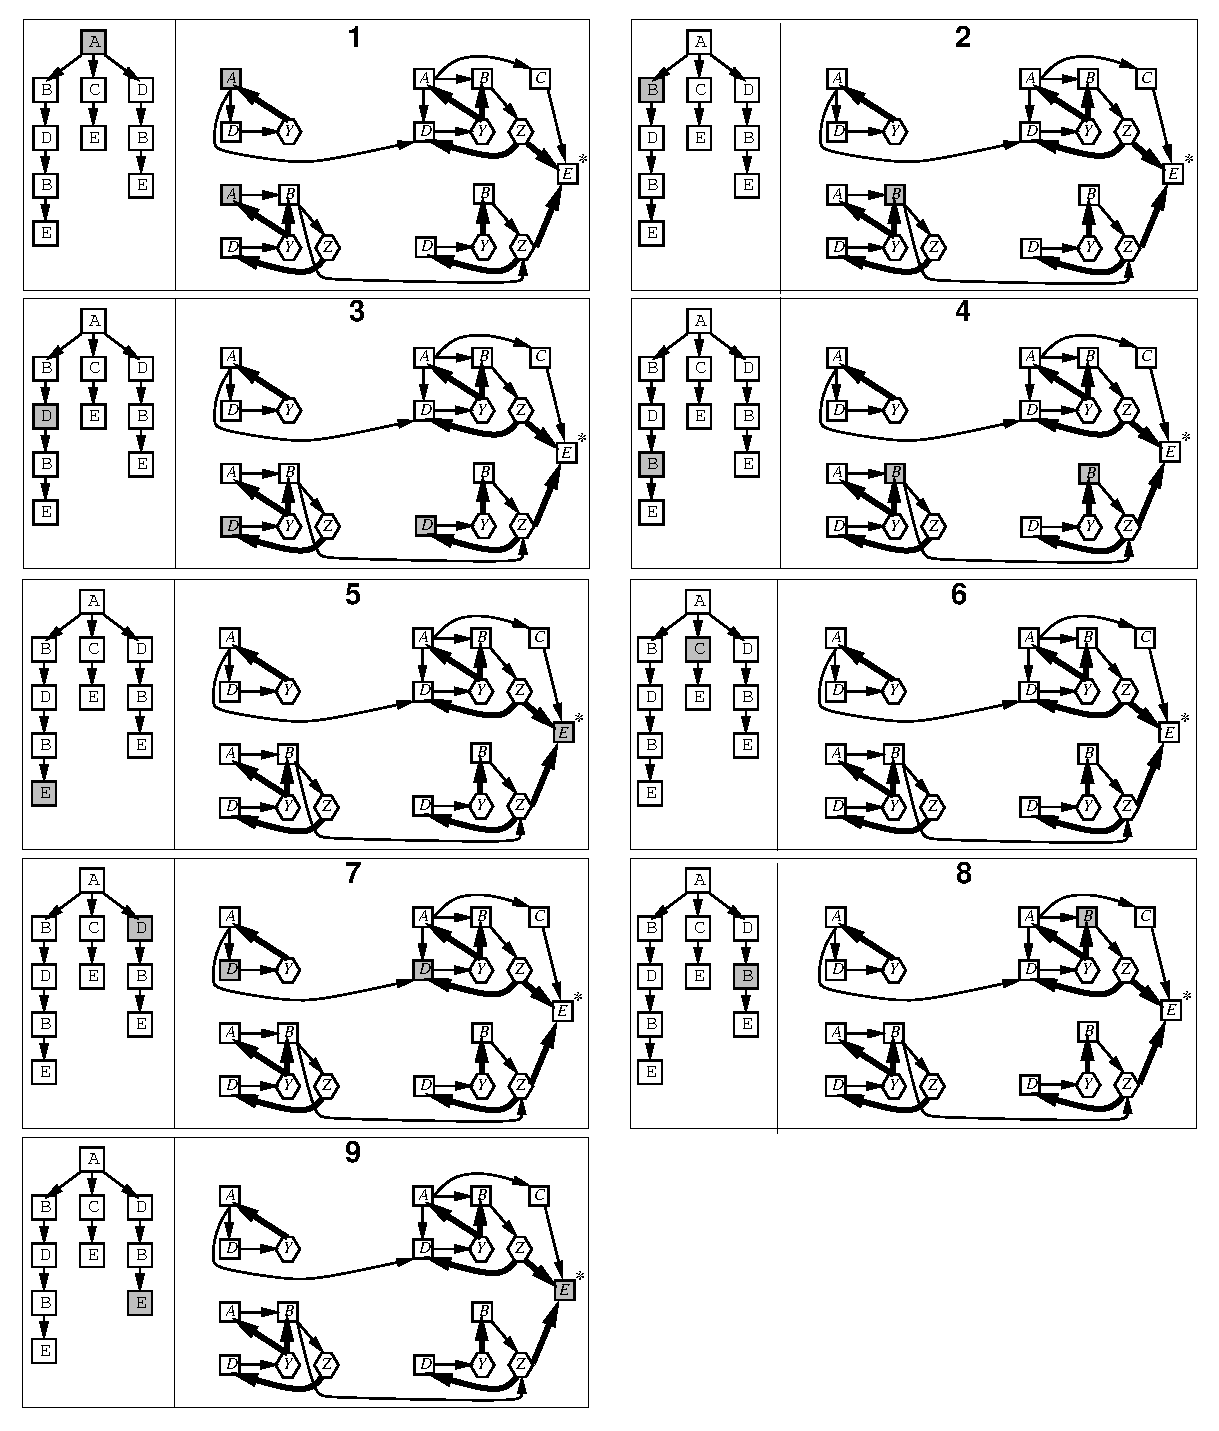
\psfig{file=run.ps,height=7.5in}}
\caption{\em
An example of an execution of traversal using the traversal of
Figure~\protect\ref{fig-comp}. At each step, the left-hand side shows
the object tree with the currently active object shaded, and the
right-hand side shows the traversal graph with the token set shaded.}
\label{fig-run}
\end{figure}

\subsubsection*{Correctness}

The following lemma states the main property of the traversal algorithm.
\begin{lemma}
\label{lem-main}
Let $\Omega$ be an object tree, and let $o$ be an object in $\Omega$.
Suppose that the $\Traverse$ methods are guided by a traversal graph
$TG$ with finish set $T_f$. Let $H(o,T)$ be the sequence of objects
which invoke {\tt visit} while $o.\Traverse(T)$ is active, where $T$
is a set of nodes in $TG$. Then
$$
\Omega\vdash_s o:X(P_{TG}(T,T_f))\rhd H(o,T)~.
$$
\end{lemma}
\Proof
By induction on $|H(o,T)|$.  For the base case, suppose that
$H(o,T)=\epsilon$. By the algorithm, this can occur only if after Step
\ref{step-abs}, $T'=\emptyset$, which means that for all concrete
nodes $v\in T$, $\Class(v)\ne\Class(o)$, and that no abstract node in
$T$ has a child whose class is $\Class(o)$.  It follows from
Definition~\ref{def-traversal} that
$\Chop(X(P_{TG}(T,T_f)),\Class(o))=\emptyset$ and hence
$\Omega\vdash_s o:X(P_{TG}(T,T_f))\rhd \epsilon$, as required.

For the induction step, assume that $|H(o,T)|>0$. Let $l_1,\ldots,l_n$
be the set of labels of traversal graph edges which start with a node
in $T'$, and let $o_i=o.l_i$ for $i=1,\ldots,n$.  In this case, by the
algorithm we have that $H(o,T)=o\cdot H(o_1,T_1)\cdots H(o_n,T_n)$,
where $T_i$ is the set of traversal graph nodes $v$ such that
$\edge{u}{l_i}{v}$ for some $u\in T'$ and such that $\edge o
{l_i}{o'}$ is an edge in the object graph.  It is follows directly
from the definitions that
$X(P_{TG}(T_i,T_f))=\Chop(\Chop(X(P_{TG}(T,T_f)),\Class(o)),l_i)$, and
hence, by the induction hypothesis, $\Omega\vdash_s
o:X(P_{TG}(T_i,T_f))\rhd H(o_i,T_i)$ and we are done.
\QED

We summarize in the following theorem.
\begin{theorem}
Let $\cS$ be a strategy, let $G$ be a class graph, let $\cN$ be a name
map, and let $\cB$ be a constraint map.  Let $TG$ be the traversal
graph generated by TGA, and let $T_s$ and $T_f$ be the start
and finish sets, respectively.  Let $\Omega$ be an object tree and let
$o$ be an object in $\Omega$.  Let $H$ be the sequence of nodes
visited when $o.\Traverse$ is called with argument $T_s$, guided by
$TG$.  Then
$$
\Omega\vdash_s o:X(\cS[G,\cN,\cB])\rhd H~.
$$
\end{theorem}
\Proof
By Lemma~\ref{lem-main}, the judgment $\Omega\vdash_s
o:X(P_{TG}(T_s,T_f))\rhd H$ holds true.  The claim of the theorem
follows from the fact that
$\cS[G,\cN,\cB]=X(P_{\TG(\cS,G,\cN,\cB)}(T_s,T_f))$ by Lemma
\ref{lem-TG}, and from the definitions of the start set $T_s$ and the
finish set $T_f$.
\QED
%
From the theorem above it is clear how to start a traversal at an
object $o$: Call $o.\Traverse$ with argument $T_s$, where $T_s$ is the
start set of the traversal.


\subsubsection*{Remarks}

\paragraph{Closed-world assumption.}  The class graph provided as
input to TGA is assumed to be the entire class graph of the program.
If an object whose class is not in $G$ is encountered while executing
TMA, even a subclass of a class in $TG$, step~\ref{step-abs} of TMA
will produce an empty $T'$, and step~\ref{step-empty} will stop the
traversal from continuing out of this instance.

\paragraph{Non-simple class graphs.}  While the class graph $G$ is
assumed to be simple, and thus the edges whose labels are in $Q$
(computed in step~\ref{step-labels}) go out of $\Class(\This)$, the
$\Traverse$ methods are equally suitable for a non-simple class graph
whose simplification is $G$, because these edges are induced
references, i.e.~fields inherited from the ancestry of
$\Class(\This)$.

\paragraph{Null references.}  Our definition of object graphs
disallows null references (though they may be simulated using
something like the Null Object pattern~\cite{null-object}), but in a
language such as Java or \C++ that permits null references,
step~\ref{step-recurse} should check that each $\This.l$ is non-null
before invoking $\Traverse$ on it.


\subsection{Computational complexity of the algorithm}
\label{ssec-analysis}
%%%%%%%%%%%%%%%%%%%%%%%%%%%%%%%%%%%%%%%%%%%%%%%%%%%%%%
It is easy to see that the time complexity of TGA is polynomial in the
size of its input.  All steps run in time linear in the size of their
input and output.  Steps~\ref{step-replicate} and~\ref{step-predicate}
take time linear in $|G'|=O(|\cS|\cdot|G|)$ and in $\tau$, where
$\tau$ is the time bound for evaluating an element predicate for a
given element.  To bound the size of the traversal graph, let $d_o$ be
the maximal number of edges going out from a node in the class graph.
Note that all edges added in Step~\ref{step-divert} correspond to
class graph edges. It follows that the number of outgoing edges added
to a traversal graph node in Step~\ref{step-divert} is $d_o$ times the
number of copies of $G$ in $G'$.  Hence Step~\ref{step-divert} may
increase the size of of the graph to $O(|\cS|^2\cdot|G|\cdot d_o)$ in
the worst case. Steps~\ref{sstep-target}, \ref{step-source}, and
\ref{step-cleanup} run in time linear in
$|G''|=O(|\cS|^2\cdot|G|\cdot d_o)$.

As for TMA, we note that the size of the argument $T$ is bounded by
the size of the strategy graph. This follows from the observation that
in all recursive invocations of $\Traverse$ made by the algorithm, for
all $v,u\in T$ we have that $\Class(v)=\Class(u)$. Since each copy of
the class graph in the traversal graph contains at most one node of
each class, it follows that the number of nodes in $T$ is never more
than the number of edges in the strategy graph.%

The proper way to describe the complexity of TMA is to express it in
terms of the number of edges in the object graph and to consider the
traversal graph size and the token set size as a constant. For each
edge in the object graph we query a traversal graph edge and when the
object graph edge is selected, we need to manipulate the token
set. The complexity of TMA is proportional to the number of edges in
the object graph.\footnote{ Note that if we allow users to call the
initial traversal with arbitrary values of $T$ (to allow multiple
sources, see Section~\ref{ssec-rem}), then it may be the case, at the
first call only, that $|T|$ is greater than the number of strategy
graph edges.  }


\subsection{Extensions}
\label{ssec-rem}
\label{sec-ext}
%%%%%%%%%%%%%%%%%%%%%%%%%%%%%%%%%%%%%%%%%%%%%%%%
\paragraph{Multiple sources and targets.}  As evident in the statement
of Lemma~\ref{lem-main}, the initial set of nodes in the traversal
graph from which the traversal starts can be arbitrary: the set of
paths traversed would change, but in accordance with the traversal
strategy, using an appropriate definition.  In particular, one may
have more than one start node in the strategy graph, which is
interpreted as several optional ``entry points'': it may be the case
that the same traversal is sometimes started with a node of class $A$
and at another time with a node of class $B$ (or, more generally, with
different nodes in the strategy graph).  Similarly, it may be the case
that we don't need all traversal paths to end with the same target
node.  This can be useful, for example, if we want to traverse a tree
of classes, rather than traverse all paths leading towards the same
target class.

This situation of multiple sources and targets can be easily handled
by our algorithm: suppose that we have a set $A$ of source nodes and a
set $B$ of target nodes for the strategy.  All we need to do is to
change Steps~\ref{sstep-target} and \ref{step-source} of TGA to be
\begin{enumerate}
\item[\ref{sstep-target}$'$.]
For each $t\in B$, add to $G'$ a node $\cN(t)^*$ and, for each edge
$e_i$ coming into $t$ in $S$, an intercopy edge
$\edge{\cN(t)^i}{}{\cN(t)^*}$.
\item[\ref{step-source}$'$.]
Add to $G'$ a node $s^*$ and, for each edge $e_i=\edge{s}{}{v}\in D$
where $s\in A$, an edge $\edge{s^*}{}{\cN(s)^i}$.  For each
$t\in A\cap B$, add to $G'$ the edges $\edge{s^*}{}{\cN(t)^*}$.
\end{enumerate}
The finish set $T_f$ is then defined to be the set of nodes $\cN(t)^*$
for all $t\in B$.

The extension to multiple targets is particularly useful when the
target of the traversal is an abstract class: suppose we want to
traverse to a class $A$ which happens to be abstract. The natural
interpretation is that the traversal should end at whatever subclass
of $A$ which happens to be in the object graph. However, with the
semantics specified above, if the target of the strategy is $A$, then
the object (whose class is concrete) substituting for $A$ is {\em not}
visited.  To visit the object substituting for $A$ regardless of its
actual class, we can simply state that the target of the strategy is
the set of all subclasses of $A$.

\paragraph{``Before,'' ``after'' and ``around'' methods.}
%%%%%%%%%%%%%%%%%%%%%%%%%%%%%%%%%%
The semantics presented in Section~\ref{sec-traversals} imposes a
pre-order of visiting the objects selected by the traversal, as
evident in TMA: first the object is verified to be on a traversal
path, then it is visited, and then the traversal proceeds down the
tree. We call such visitor methods {\em before visitor methods}.  It
is sometimes useful to have the visitor methods invoked in post-order,
namely first descend down the tree and then invoke the visitor
method. These visitor methods are accordingly called {\em after
visitor methods}. It is a simple exercise to adapt the definition of
traversals to deal with after visitor methods.

Both before and after visitor methods are generalized by the notion of
{\em around visitor methods}, whose code is interleaved with the
traversal method code of TMA.  This allows for before and after
methods (which can communicate directly by shared data structures),
and it also allows the visitor to directly manipulate the traversal,
e.g., by invoking it multiple times, or by pruning it.
 
\paragraph{Cyclic object graphs.}  One of the apparent disadvantages
of the approach presented in the current paper is that it deals only
with tree (or forest) object graphs.  This problem can be solved in
many ways, depending on the intended semantics. In the current
implementations, we use visitor methods to make sure that a visited
node is not revisited in directed acyclic or in cyclic object graphs.
The main point is that we already have all the machinery to carry out
a depth-first traversal of a part of the object graph as selected by
the strategy, so it is quite easy to vary the implementation slightly
to accommodate for our needs. In a sense, what we need is a
specialized around method (see above).

For example, one reasonable choice is that no object is visited
twice. This can be easily implemented by associating a ``{\tt
visited}'' bit with each object (or alternatively a hash table), and
using it as expected, namely to execute the following as the first
step in the traversal method (TMA) (initially, $o.\mbox{\tt
visited}=\False$ for all objects $o$):

\begin{enumerate}
\item[0.] 
If $\This.\mbox{\tt visited}=\True$, return. 
Else $\This.\mbox{\tt visited}\gets\True$.
\end{enumerate}

\section{The limits of static traversal code}
\label{sec-lb}
%%%%%%%%%%%%%%%%%%%%%%%%%%%%%%%%%%%%%%%%%%%%%%%%%
One appealing approach to compiling executable code from traversal
strategies is to use only static analysis: in this context, this means
that only method invocations are used to traverse the graph, with no
further computation while the program is running. The advantage of the
static approach is that the run time overhead due to traversals is
minimal; the possible disadvantages are larger compile time and higher
space requirement for the executable code, but how large can they be?
Early implementations of traversals were static, but they suffered
from either being limited in scope~\cite{lieber-palsberg-xiao94,
gener-comp-j:jens-boaz-karl}, or inefficient.  in particular, the
automata-based algorithm presented
in~\cite{gener-comp-j:jens-boaz-karl} may result in exponential
compilation time and exponential number of traversal methods in the
executable code.

In this section we show that this phenomenon is not accidental: for
some strategies and class graphs, static compilation algorithms must
output exponentially many methods, thereby making the space
requirement of the code, as well as the running time of the compiler,
infeasible in the worst case.  We remark that our proof technique is
similar to the standard technique of simulating non-deterministic
finite automata in polynomial space and time~\cite{dragon-nfa-sim}.

To state the result formally, we first define the notion of static
traversal compilation. We then give an example of a traversal strategy
and a class graph where static compilation must result in an
exponential number of methods.  We remark that the strategy graph we
use is not cyclic; in fact, a tree strategy is sufficient to prove the
same result.


\subsection{The target language}
%%%%%%%%%%%%%%%%%%%%%%%%%%%%%%%%
An algorithm is said to compile a traversal strategy and a class graph
to {\em static traversal code} if it generates traversal code in a
language which supports only method invocation without parameter
passing.  The target language of a static compilation algorithm is
formally defined in~\cite{lieber-palsberg-xiao94,
gener-comp-j:jens-boaz-karl}, and is given in
Appendix~\ref{sec-target}.  Informally, a program attaches method
definitions to each class, and a method body is a list of (qualified)
method names. There are no arguments passed to the methods and no
return values.  Executing a method in a given object graph is done
simply by unfolding the method definition. To perform a traversal
starting with a given object, a special method attached to this object
is invoked. When a method is invoked, the corresponding object may be
added to the traversal history.

\subsection{The lower bound}
%%%%%%%%%%%%%%%%%%%%%%%%%%%%
We now prove the main result of this section.
\begin{theorem}
\label{thm-lb}
For any $n>0$ there exists a traversal strategy $\cS_n$ with
$|\cS_n|=O(n)$ and a class graph $G_n$ with $|G_n|=O(n)$ such that the
number of methods in a static traversal code corresponding to $\cS_n$
and $G_n$ is at least $2^n$.
\end{theorem}
\begin{figure}
\newlength{\figwidth}
\setlength{\figwidth}{\textwidth}
\addtolength{\figwidth}{-5mm}
\centerline{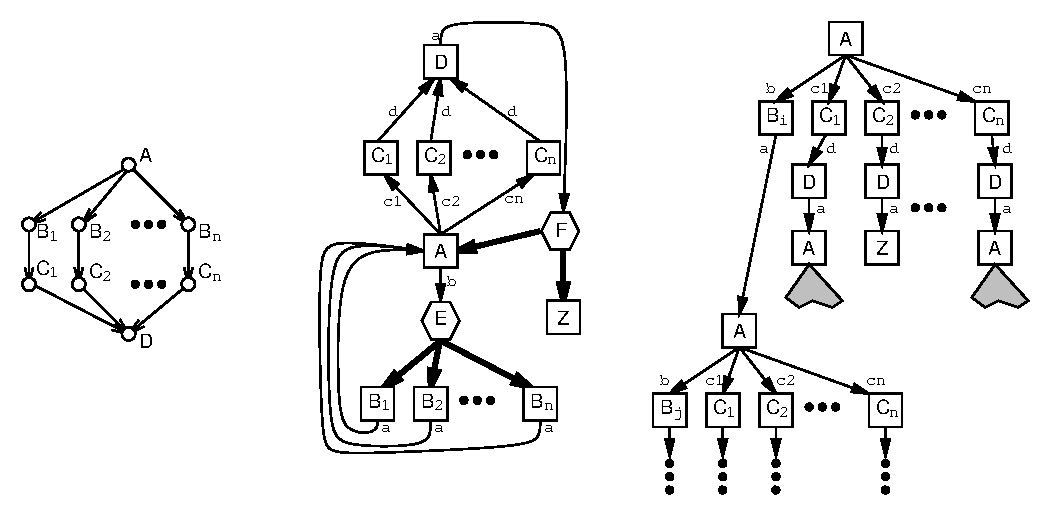
\psfig{file=lb.ps,width=\figwidth}}
\caption{\em 
Example considered in lower-bound proof.  Left: the strategy
graph. The source of the strategy is the node labeled {\sf A} and the
target is the node labeled {\sf D}.  Middle: the class graph. The name
map is indicated by the node labels on the strategy graph. Right: a
typical object tree. The shaded regions represent a recursive
occurrence of the tree.  }
\label{fig-lb}
\end{figure}
\Proof
By contradiction.  Consider the strategy graph and the class graph
depicted in Figure~\ref{fig-lb}. Intuitively, starting with an object
of class $A$, an object of class $C_i$ can be visited only if it has
an ancestor of class $B_i$.  The strategy graph has $2n+2$ nodes and
$3n$ edges; The class graph has $2n+3$ nodes and $4n+2$ edges.  Note
that we can construct object trees where an $A$-object has any desired
set of $B$-ancestors.  We claim that in a static traversal code, there
are at least $2^n$ methods attached to objects of class $A$.  For
suppose not.  Then there exists a set
$S_0\subseteq\Set{C_1,C_2,\ldots,C_n}$ such that there is no method
attached to $A$ which consists of calls precisely to the methods in
the objects pointed to by the elements of $S_0$. Let $I_0$ be the set
of indices in $S_0$.  Consider an object tree containing an object $o$
with $\Class(o)=A$ such that $o$ has an ancestor of class $B_i$ if and
only if $i\in I_0$. Put differently, we think of an object tree which
satisfies the following condition: $$
\Set{\Class(o')\mid o' \mbox{ is an ancestor of }o}\cap
\Set{B_1,B_2,\ldots,B_n}= \Set{B_i\mid C_i\in S_0}~.
$$
As noted before, such an object graph exists.  By definition, when $o$
is invoked, it should call precisely those children whose class is in
$S_0$. But by assumption, no such method is attached to $A$.
\QED

We note that the strategy graph in the proof of Theorem~\ref{thm-lb}
is acyclic (in fact, it is a series-parallel graph expressible in the
syntax for traversal specifications of
\cite{gener-comp-j:jens-boaz-karl}).  The proof extends directly to
the case of tree strategies (see Section
\ref{sec-ext}) by omitting the node corresponding to $D$ in the strategy
graph.

It may be instructive to see how the algorithm described in Section
\ref{sec-alg} avoids the exponential lower bound. In that algorithm,
the traversal graph serves as a ``road map,'' and whenever a traversal
method is called in an object $o$, it gets as an input argument a set
of ``tokens.''  The token set reflects the current location of the
traversal, i.e., what prefixes of paths have already been covered when
the traversal reached $o$.  This set controls the next traversal
actions while being updated as the traversal continues.  As the
argument of Theorem~\ref{thm-lb} implies, the number of possible
continuations of the traversal may be exponential; however, this only
means that the number of possible configurations of the token set must
be exponential, which can be achieved with an argument whose size is
linear in the size of the strategy graph.

\section{Implementation notes}
\label{sec-notes}
%%%%%%%%%%%%%%%%%%%%%%%%%%%%%%%

In this section we describe some of the practical issues and design
decisions taken in the course of development of the Demeter
software~\cite{URL:demeter}, based on the idea of traversal strategies
as described in this paper.

\subsection{User-level representation}
\label{ssec-syntax}
%%%%%%%%%%%%%%%%%%%%%%%%%%%%%%%%%%%%%%%
%To aid specifying inputs, the system contains a graphical editor which
%allows the user to enter class and strategy graphs via an intuitive
%interface. The idea is that the class graph is either generated
%automatically from a given Java code, or that the user draws it
%manually. The representation we use is similar to that of UML
%\cite{grady-jim:95}. In the next step, the user specifies a strategy
%graph by pointing at the class graph nodes. This method, aside for the
%obvious ease-of-use, also implicitly defines the name map: a strategy
%node is mapped to the class node from which it was derived.  The
%constraint map predicates are defined by clicking on the undesired
%elements.

%In addition to the graphical representation,
An LL(1) grammar has been developed to support textual representation
of strategies.  The syntax of strategies is given as an edge list
between curly brackets, with the source and target nodes prefixed with
{\sf source:} or {\sf target:}, respectively.  The default name map
associates a strategy node with a class with the same label.

Example:
\begin{quote}
\begin{verbatim}
{ source: A -> B    B -> C    C -> target: D }
\end{verbatim}
\end{quote}
If a strategy's graph is a line graph, we may also use 
from--via--to syntax; the above strategy could also be written as:
\begin{quote}
\begin{verbatim}
from A via B via C to D
\end{verbatim}
\end{quote}

In fact, the textual representation is a much more effective way to
specify the constraint map.  Specifically, each strategy edge may be
followed by an element predicate expressed with any of the following
forms:
\begin{quote}
\begin{verbatim}
 bypassing { A, B }
 bypassing -> *,l,*
 only-through -> A,l,B
\end{verbatim}
\end{quote}
The first predicate is true for all elements except for nodes {\sf A}
and {\sf B}.  The second predicate is true for all elements except for
edges whose label is {\sf l}. The third predicate is false for all
elements except for the edge $\edge{\mathsf A}{\mathsf l}{\mathsf B}$.

The expression for the strategy given in pane 2 of Figure~\ref{fig-comp},
including the constraint map, is given below:
\begin{quote}
\begin{verbatim}
{ source: A -> D           bypassing -> B,z,Z
          D -> target: E
          A -> Z           bypassing -> A,d,D
          Z -> E           bypassing A         }
\end{verbatim} 
\end{quote}

\subsection{Tool responsibilities}
\label{ssec-tools}

The Demeter software~\cite{URL:demeter} includes several different
tools and libraries, all using the technology described in this paper.
We briefly describe the responsiblities of those tools, how they
relate, and what their limits are.

\subsubsection{AP Library}

The AP Library is a Java implementation of TGA.  It includes a set of
Java interfaces and default implementations (including parsers) for
the concepts of class graphs, traversal strategies, name maps, and
constraint maps, as well as a {\sf Traversal} class that represents a
traversal graph constructed from these four objects.  The AP Library
includes a number of enhancements to the basic structures and
algorithms defined in this paper; one recent enhancement is the
ability to intersect two strategies, which is efficiently implemented
by computing two traversal graphs which can be traversed in parallel,
only moving ahead in the object graph when both traversal graphs allow
it.  More details about this and other enhancements will appear in a
future paper.

\subsubsection{DJ}
\label{ssec-DJ}

The idea of the DJ library~\cite{OrleansLieberherrReflection01,
adaptive-methods-cacm-2001} is to add traversal strategies to
Java without extending the language; instead, traversal is done using
an API that computes traversal graphs at runtime (using the AP
Library) and interprets them using TMA.  A vector of {\sf Visitor}
objects can be carried along the traversal to perform behavior along
the way.  The Java Reflection API is used to create class graphs,
traverse object graphs, and invoke visitor methods.  

DJ also integrates generic programming with adaptive programming.  DJ
supports the adaptive definition of iterators that are used by generic
algorithms.  The tool works with the Java collection classes and
offers the capability to use strategies to view an object graph as
a list even though the paths to the objects in the list may be complex.

\subsubsection{DemeterJ}

DemeterJ~\cite{cse:preventive}, is our oldest Java tool improving on
our \C++ implementation described in~\cite{karl:demeter}.  DemeterJ
takes as input a class dictionary file and a set of behavior files,
which contain plain Java methods, traversal strategies, and visitor
methods.  It then generates Java source code for the traversals that
implements TMA, invoking the visitor methods along the way.  DemeterJ
is often used after a project has been prototyped using the DJ library
because DemeterJ generates traversal code, which is faster than
traversing with reflection.

The class dictionary syntax is a concise way of defining a class
graph, including its fields and accessor methods.  For example, the
class dictionary for the class graph of pane 1 of
Figure~\ref{fig-comp} can be expressed as follows:
\begin{quote}
\begin{verbatim}
A = "a" <b> B <c> C <d> D.
B = "b" <z> Z.
D = "d" <y> Y.
C = <e> E.
Y : A | B.
Z : D | E.
E = "e".
\end{verbatim} 
\end{quote}
Essentially, the graph is represented as a list of nodes, where each
node is represented by a list of its outgoing edges, with the edge
labels in angle brackets.  The class dictionary is annotated with some
syntactic sugar in double quotes to make an LL(1) grammar which is
used to generate a parser that creates an object graph for a given
input sentence.  For example, assuming the above class dictionary, the
object graph in Figure~\ref{fig-run} can be created with the following
Java code:
\begin{quote}
\begin{verbatim}
A a = A.parse("a b d b e e d b e");
\end{verbatim}
\end{quote}

DemeterJ also generates several utility visitors from a class
dictionary, such as for printing, copying, or comparing object graphs
or tracing traversals.

\subsubsection{DAJ}

DAJ~\cite{URL:DAJ,sung:DAJ-02} is our latest tool and it takes
AspectJ~\cite{aop:ecoop2001}, rather than Java, as the starting point.
DAJ performs a similar task as DemeterJ, taking as input a set of
class dictionaries and aspects (augmented with declarations of
strategies and traversals) and using the AP Library to generate
traversal code that implements TMA.  Integrating with AspectJ allows
the user to benefit from both adaptive programming and aspect-oriented
programming~\cite{cacm-2001} in the same program.  All of the
current features of DemeterJ will eventually be available in DAJ, and
future development will be geared towards enhancing DAJ, DJ, and the
AP Library.

See Section~\ref{sec-appls-trav-strats} for other ways traversal
strategies can fit into AspectJ.

\section{Related work}
\label{sec-related}
It is surprising to see that despite the universality of traversals in
programming, only very little work has been done in this direction,
although the pace is picking up.  Until recently, the automation of
traversal of object structures using succinct representations has been
unique to Demeter (\cite{lieber-nacho-cun:pp-cacm}, see above); the
rising popularity of markup languages in general, and XML in
particular, created a new interest in traversals. In this section we
list some work relevant to traversals.

XML is a new standard for defining and processing markup languages for
the web~\cite{XML}.  XML uses grammars (also called {\em document type
definitions} or {\em schemas\/}) to define a markup language for a
class of documents.  To select subsets of XML document elements, the
W3 Consortium recently introduced a language called XPath
\cite{XPath}.  The way elements are selected in XPath is by
navigation, somewhat resembling the way one selects files from an
interactive shell, but with a much richer language.  Recently
\cite{XPath-traversals}, XPath has been proposed as input to a
universal object model walker for arbitrary Java objects.  XPath
expressions are used to describe {\em sets of objects}, in the sense
that the value of an expression is an {\em unordered} collection of
objects {\em without duplicates}. This is in contrast to traversals,
whose value is a set of {\em paths}, so that the objects of each path
are explictly ordered and may appear more than once, even on the same
path. It is quite easy to implement XPath using strategies, using
specialized ``visitors.'' The converse, however, does not hold, due to
the lack of structure in XPath expression values.  While XPath is a
powerful language to address parts of an XML document, there are cases
in which strategies can be used to select the same sets with {\em
exponentially} shorter representation than the representation of
XPath.

A bad example for XPath is (currently) as follows (XPath is in the
process of being extended moving closer to the traversal strategy
model to make this also easily expressible). Take a strategy graph
with start node $S$ and target node $T$ and nodes $A_i$ and $B_i$ for
$i$ from 1 to $n$ and nodes $C_j$ for $j$ from 1 to $n-1$.  There are
edges from $S$ to $A_1$ and $B_1$; from $C_i$ to $A_{i+1}$ and
$B_{i+1}$ and from $A_i$ and $B_i$ to $C_i$ for $i$ from 1 to $n-1$;
from $A_n$ and $B_n$ to T.  Note that there are exponentially many
paths from $S$ to $T$ and if we want to express the $T$ nodes that we
want to select in XPath, we have to enumerate all those paths using
the XPath notation. The size of the strategy graph solution is linear,
while the size of the XPath solution is exponential.

This example may lead to exponential running times for some input
objects both for the XPath and the traversal strategy case.  It is the
responsibility of the programmer to recognize this possibility and
deal with it using appropriate visitor objects.

In the context of {\em object-oriented databases}, traversals are
heavily used. Some automation of traversal was suggested in
\cite{ns:vldb88,bv:navigation,MarSho:abbrev-query-int93,querying-oodb:kim92,ioannidis:path-expr}.
Roughly speaking, the idea in these papers is to traverse to a target
without specifying the full path leading to it.  Cast in our terms,
one can view these techniques as a variant of line-graph strategies
(i.e., strategy graphs with a single path) ; however, their goal is to
allow the user to abbreviate the laborious specification of a full
query, and their main concern is how to complete the abbreviation when
it is ambiguous, sometimes using heuristics.  Another complication
these approaches confront is that queries are specified on-line and
can therefore refer to run-time structures.  By contrast, our approach
ignores the ambiguity problem by traversing all qualified objects, and
requires traversal specifications to refer only to compile-time
structures. On the other hand, strategies allow for general graph
specification, and entail (when combined with visitors) the power of a
full-fledged programming language.

In the context of programming languages, traversals are frequently
used as a part of {\em attribute grammars}, for traversing abstract
syntax trees~\cite{WaiteGoos84}.  Using conventional programming
techniques, the details of traversals must be hard-coded in the
attribute grammar; this fact makes attribute grammars hard to
maintain, say in the case of some modifications in the grammar
\cite{kastens:waite}.  In the Eli system~\cite{ELI}, this problem is
addressed by separating the details of the grammar from the underlying
algorithm, using traversal specifications which basically correspond
to single edge strategy graphs.  There are papers dealing with a more
modular, component-based approach to attribute grammars, such as
\cite{composable-attribute-gr:popl92}. This allows traversals for
different aspects or phases to be separated, partially addressing the
concerns of scattering and tangling of traversal code.  However, the
mapping from specific attribute grammars to high-level attribute
grammars needed in a modular attribute grammar approach could be
expressed more conveniently with traversal strategies.

Meta-programming techniques have also been developed for
traversals. For example, in~\cite{cameron-ito:gramps}, a simple kind
of traversal (corresponding to a one layer tree graph) is used in a
meta-program; this traversal scans all objects and executes the
specified code at the desired targets.

{\em Strategic programming} (SP)~\cite{LVV:strategic-programming}
provides the programmer with full traversal control with {\em
traversal schemes} that can be built up modularly using a rich set of
combinators.  A key difference between SP and AP is that traversals in
SP may follow paths in an object graph that can never lead to target
classes; no reachability computation is done.  In general, this is
undecidable in SP, because the traversal combinators form a
Turing-complete language.

The {\em Visitor} design pattern is discussed in many
software-engineering works (e.g.,~\cite{gang-of-4}). While this
approach identifies and isolates the task of traversal, no mechanism
to automate the task and make it adaptive was previously
proposed. Moreover, no formal treatment of traversal was offered.  As
a side remark from the software engineering perspective, we note that
our approach of separating the traversal task from the class-structure
of an object oriented program can be viewed as a special case of {\em
aspect-oriented programming}~\cite{cacm-2001}, where the idea is to try
to align different conceptual aspects of programming with actual code
modules.

Visitor generators have been around for a while (e.g.,
\cite{palsberg:jay,stirewalt01generation,bravenboer01guiding}),
usually generating a default DepthFirst visitor with before and after
hooks. Since these visitors only need to be manually specialized for
selected types of the visited class hierarchy, they are adaptive to
some degree. But visitor generators fall short of the accomplishments
of our approach for the following reason: They don't take advantage of
a high-level approach to specifying traversals and instead the
generated visitor goes everywhere. For example, to implement a
traversal {\sf ``from A to B''} with a visitor generator, we would
have to specialize the visitor manually for all classes between A and
B where we don't need to visit all outgoing edges. A visitor generator
generates traversals of the form {\sf ``from A to *''} and then we
have to simulate bypassing clauses using subclassing.

An important tool for aspect-oriented programming is AspectJ from
Xerox PARC~\cite{aop:ecoop2001}. Generally speaking, AspectJ allows the
programmer to manipulate {\em pointcuts}, which are a collection of
points in the execution. In Section~\ref{sec-appls-trav-strats} we
describe two applications of traversals to AspectJ. A traversal
defines a structured set of join points (calls of the traversal
methods) while in AspectJ a much richer set of join points is used.
Visitors are advice on the traversals.

The idea behind succinct specifications of mathematical structures
\cite{galperin:wigderson} is to exploit regularity. If there is no
regularity, succinctness will not work.  In~\cite{galperin:wigderson}
boolean circuits are used to represent graphs succinctly.  We instead
use traversal strategies to define subgraphs succinctly.

\section{Comparison to traversal specifications}
\label{sec-comparison}
\newcommand{\OLD}{$\cL_{\mathrm{OLD}}$}
\newcommand{\NEW}{$\cL_{\mathrm{NEW}}$}

In this section, by \OLD\ we mean the traversal specification language
of~\cite{karl:comp-enh,lieber-palsberg-xiao94} and by \NEW\ the traversal
specification language for strategies presented in this paper.

The comparison between \OLD\ and \NEW\ is delicate but \NEW\ is an
important improvement over \OLD. Some traversal specifications are
equally easy to express in \OLD\ as in \NEW, other \NEW\ traversal
specifications are impossible to express in \OLD\ and some traversal
specifications expressed in \NEW\ can be expressed in \OLD\ but are
exponentially longer.

We discuss the following three points in detail:
\begin{enumerate}
\item Any traversal specification in \OLD\ is a directed
      series-parallel graph~\cite{eppstein92parallel} and can be
      expressed as a strategy in \NEW.  In other words, we have upward
      compatibility.  Example: The \OLD\ style traversal specification
\begin{tabbing}
[{\sf Company},{\sf Domestic}]$\cdot$%
(\=[{\sf Domestic},{\sf ServiceIncome}]$\cdot$%
   [{\sf ServiceIncome},{\sf Money}]\\
\>+[{\sf Domestic},{\sf GoodsIncome}]$\cdot$%
   [{\sf GoodsIncome},{\sf Money}])
\end{tabbing} is expressed as the strategy shown in
Figure~\ref{fig-company-strat1}.  The translation maps each
``from-to'' part of the form [$X$,$Y$] to an edge in the strategy.
\begin{figure}
\centerline{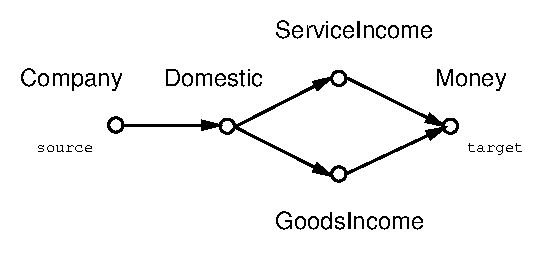
\psfig{file=companystrat1.ps}}
\caption{\em A series-parallel traversal strategy.}
\label{fig-company-strat1}
\end{figure}

\item Some of the traversal specifications in \OLD\ can be expressed
      much more succinctly as a strategy in \NEW.  Consider the
      following \OLD\ traversal specification
\begin{tabbing}
[{\sf Company},{\sf Domestic}]$\cdot$%
(\=[{\sf Domestic},{\sf ServiceIncome}]$\cdot$%
   [{\sf ServiceIncome},{\sf Money}]\\
\>+[{\sf Domestic},{\sf GoodsIncome}]$\cdot$%
   [{\sf GoodsIncome},{\sf Money}])\\
+[{\sf Company},{\sf Foreign}]$\cdot$[{\sf Foreign},{\sf GoodsIncome}]$\cdot$[{\sf GoodsIncome},{\sf Money}]
\end{tabbing}
which duplicates [{\sf GoodsIncome},{\sf Money}].  The traversal
specification will traverse to all {\sf Money} objects. The domestic
and the foreign parts of the company are treated differently: for
domestic parts we traverse both into {\sf ServiceIncome} and {\sf
GoodsIncome} while for foreign parts we traverse only into {\sf
GoodsIncome}. In the corresponding traversal strategy given in
Figure~\ref{fig-company-strat2}, this duplication is not needed.
\begin{figure}
\centerline{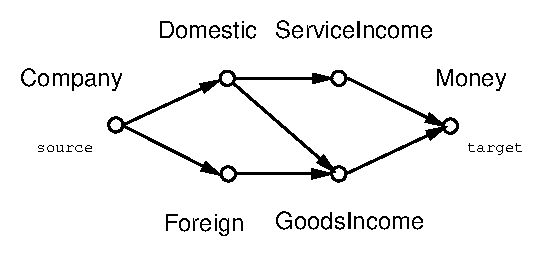
\psfig{file=companystrat2.ps}}
\caption{\em A non-series-parallel traversal strategy.}
\label{fig-company-strat2}
\end{figure}

Remembering the motivation that a traversal strategy with source $s$
and target $t$ defines a set of paths from $s$ to $t$, we can always
replace a strategy that is a dag by a set of paths that are merged
together.  Because the number of paths from $s$ to $t$ may be
exponential in the size of the dag and there may be no shorter
possibility than enumerating all of them, the old representation may
be exponentially longer.  Consider the following strategy with $n$
nodes $ A_1, A_2, \ldots, A_n $. There are edges
$\edge{A_i}{}{A_{i+1}}$ for $ i = 1, \ldots, n-1 $ and edges
$\edge{A_i}{}{A_{i+2}}$ for $i =1, \ldots n-2 $.
Figure~\ref{fig-expstrat} shows this strategy with $n=7$.
\begin{figure}
\centerline{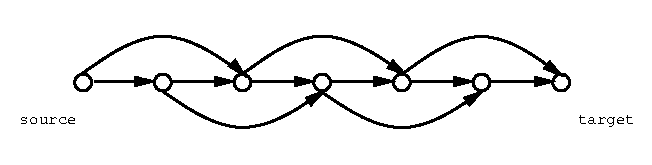
\psfig{file=expstrat.ps}}
\caption{\em A non-series-parallel strategy with $n$ nodes and $O(2^n)$ paths
($n=7$ here).}
\label{fig-expstrat}
\end{figure}
The resulting graph is not series-parallel and the only way to express
the set of paths from source $ A_1 $ to target $ A_n $ using only join
and merge is to enumerate a number of paths that grows exponentially
in $n$.  We can use a series-parallel construction for some of the
paths but overall we will have an exponential number of paths and
therefore a traversal strategy that grows exponentially in $n$.

\item There are cyclic strategies (expressed in \NEW) which cannot be
simulated by \OLD.  Consider the following traversal that cannot be
simulated by a traversal specification in \OLD. For a given city, we
want to find all other cities reachable through zero or more bus
routes. Consider this specification in the context of the class graph
in Figure~\ref{fig-citycd}.
\begin{figure}
\centerline{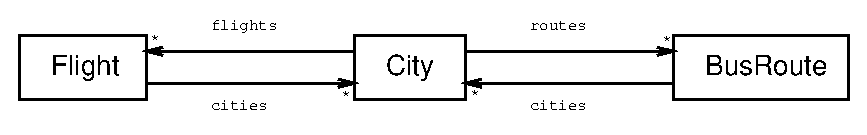
\psfig{file=citycd.ps}}
\caption{\em Class graph for a transportation network.}
\label{fig-citycd}
\end{figure}
Using this class graph, we can start at a city and follow paths of the
form $$\Seq{\mathsf{City\ }(\mathsf{routes\ BusRoute\ cities\
City})^*}$$ to find all cities connected to it by bus routes only. We
are not interested in the cities reachable through flights. We can use
the cyclic strategy shown in Figure~\ref{fig-cyclic-strategy}, which
\begin{figure}
\centerline{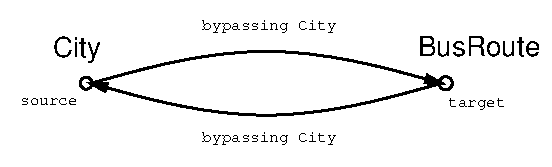
\psfig{file=cyclicstrat.ps}}
\caption{\em A cyclic strategy.}
\label{fig-cyclic-strategy}
\end{figure}
selects the desired {\sf City} objects. But this cyclic strategy
cannot be expressed by a series-parallel graph.  We could try:
\begin{verbatim}
from City bypassing City via BusRoute bypassing City to City
\end{verbatim}
but this allows only cities reachable through an immediate
bus route.

\end{enumerate}

To summarize: the new language is exponentially more expressive in
some cases and combined with the exponential algorithmic improvement
presented in this paper the new approach is considerably more
efficient than the old approach.

\section{Applications of traversal strategies}
\label{sec-appls-trav-strats}

This paper focuses on succinctly definining behavior for traversing
through object graphs and on efficient implementations of the
traversals. However, our traversal theory (the expressive model and
the efficient algorithms) is applicable in a much wider context which
we outline in this section.

The traversal theory relies on three layers of graphs: top, middle and
bottom. The bottom layer consists of trees that we want to traverse to
select subtrees. Each bottom layer tree has a graph from the middle
layer associated with it that contains meta-information about the
bottom layer tree. The meta-information expresses that certain edges
must or may exist. Each middle layer graph is associated with at least
one top layer graph. The top layer graph is basically a subgraph of
the transitive closure of the middle layer graph, decorated with
additional information attached to the edges. The purpose of the top
layer graph is to define subtrees of the bottom layer graphs. In
other words, when the bottom layer graph is traversed, the top layer
graph tells us at each node which outgoing edges to traverse.  The
purpose of the middle layer graph is to act as an abstraction barrier
between the top and bottom layers. At the middle layer we program the
specification given by the top layer and we use the middle layer to
reduce the search space.

The top layer graphs are an abstraction A of the associated middle
layer graphs and the middle layer graphs are an abstraction B of the
associated bottom layer graphs. The abstractions A and B, however, are
different. Abstraction A involves the transitive closure and
abstraction B involves compatibility rules where relations at the
middle layer imply relations at the bottom layer.

The traversal theory is also useful if we only use the top and the
middle layer. In this case we are interested in defining succinctly a
set of paths in the graph in the middle layer. Sometimes we are not
interested in the details of the path set, just the subgraph or set of
nodes that all those paths in the set cover.

This general description fits many practical situations of which we
mention a few, all of them of interest to aspect-oriented programming.

\begin{itemize}
\item 
The standard application: Top: strategy graph, Middle: class graph,
Bottom: object trees. The strategy graph serves as a specification of
a set of introductions of new traversal methods into the class graph.
This standard application is used extensively in DemeterJ and DAJ.  DJ
also falls into this standard application, however, the traversal
behavior is created at run-time by specializing a generic traversal
algorithm.

If we focus on the top and middle layer only, we need only our
Traversal Graph Algorithm (TGA) described in Section~\ref{ssec-TG}.
One application of TGA is to use it to succinctly specify a set of
types. In AspectJ, type patterns could benefit from using strategies
to specify a set of types succinctly.

A second application of TGA is the adapter generation approach by Bart
Wydaeghe and Wim Vanderperren
\cite{bart:thesis02,bart-wim:strategies-ref,vanderperren:composition-adapters}.
The components that need to be connected might not match and therefore
an adapter has to be generated. The idea is that a traversal graph
that is constructed by TGA succinctly describes all possible adapters
from which the programmer can choose the most suitable one. The top
layer graph represents the interactions of a high-level component and
the middle layer graph represents the interactions of a low-level
component that offers more detail than the other component asks for.
The PacoSuite is a tool in which those ideas have been successfully
implemented and tested in an industrial context. The application uses
the full power of traversal strategies, including bypassing clauses
and the name maps.

\item The call graph application: Top: computational pattern, Middle:
static call graph, Bottom: call tree.

Static call graph: It is derived from the program source as
follows. The nodes correspond to methods and the edges to method
invocation expressions (e.g.\ {\sf a.foo(b,c)}) contained in the
methods. There are two types of methods: concrete and abstract. A
concrete method has an outgoing edge for every method the method calls
or might call. Some of the outgoing edges are marked required and
others are marked optional. The required edges are to calls of other
methods that are reached unconditionally while optional edges
correspond to calls that are reached conditionally (some conditional
statement might prevent the execution of the call; e.g. an if, loop or
switch statement). An abstract method has several outgoing edges
marked as virtual edges. Each leads to one of the method calls that
might happen as a result of the virtual method call. A static call
graph has the shape of a class graph.

Dynamic call tree: It is a tree conforming to a static call graph. The
nodes are calls of methods (called join points) and the edges
represent immediate method call nesting. Conformance means that
\begin{enumerate}
\item the dynamic call graph can only contain instances of call sites
      appearing in the static call graph;
\item the dynamic call graph can only contain edges prescribed by the
      static call graph;
\item if in the static call graph a required edge exits a call site
      then the edge must be in the dynamic call graph; and
\item a call of a virtual method is not shown in the dynamic call
      graph; instead it shows the concrete method that actually gets
      called.
\end{enumerate} 
A dynamic call tree has the shape of an object tree where call nodes
correspond to object nodes and immediately nested calls correspond to
immediately nested objects.

As an example, consider the set of all method calls that might happen
between a call to {\sf f} and a call to {\sf g}. For each of those
method calls we would like to print some information and we would like
to know how the join points are related. In other words, we want to
know the structure of the dynamic call tree between calls to {\sf f}
and calls to {\sf g}. We would like to describe this slice of the
dynamic call tree as {\sf from pc1 to pc2}, where {\sf pc1 = call(*
f(..))} and {\sf pc2 = call(* g(..))}.  (The pointcuts {\sf pc1} and
{\sf pc2} specify that both {\sf f} and {\sf g} may return any type
and both may have arguments of any types.)

In a second example, we want to know for a thread and a resource type
{\sf R} all the {\sf read}, {\sf write}, {\sf lock}, and {\sf unlock}
calls that happen during the thread.  Furthermore, we want to check
that none of those primitives call each other; for example, we want to
disallow that {\sf write} calls {\sf lock} directly.

We consider four kinds of nodes in the static call graph corresponding
to calls of the four primitives.
\begin{quote}
\begin{verbatim}
pointcut read(): call(Object R.read(..));
pointcut write(): call(void R.write(..));
pointcut lock(): call(void R.lock(..));
pointcut unlock(): call(void R.unlock(..));
pointcut primitive(): read() || write() || lock() || unlock();
\end{verbatim}
\end{quote}

The pointcut {\sf start} contains a node in the static call graph
where the computation starts.  We consider the following two
strategies:
\begin{quote}
\begin{verbatim}
s1 = from start() to primitive()
s2 = from start() bypassing primitive() to primitive()
\end{verbatim}
\end{quote}
(Note that bypassing a node does not bypass that node if it is a
start or end point.)

The primitives don't call each other iff, for the given static call
graph, {\sf s1 = s2} (more precisely, if the traversal graphs
determined by the two strategies are equal).  This second example is
interesting because it shows that strategies are useful to formulate
architectural properties of call graphs at a high level of
abstraction.
\end{itemize}

Finally, we present a use of the call graph application in
serialization/marshalling which is a very common example of object
traversal.  A serializer is a tool transforming partial graphs of
objects into a stream of bytes.  In~\cite{Lopes96a}, simple traversal
directives (which are single edge strategy graphs) are used to specify
which parts of a compound object should be copied and which should be
passed by reference when using remote method invocations.  Our work on
traversals is useful to current work in object serialization
\cite{phillipsen:CPE,bartoli:SPE,hoschka:marshalling} in the following
way: A common concern in serialization is how to generate
serialization code with minimal impact on the code size of the
application, or alternatively, how to arrange dynamic traversal with
minimal run-time impact.  We address this concern by showing in
Section~\ref{sec-lb} that if the traversal methods are not generated
carefully from a partial object specification (as described in this
paper), one might end up with exponential code size.  Our
implementation of DJ shows how to arrange dynamic traversal and the
DemeterJ and DAJ implementations show how to generate efficient code
efficiently.  We also show a general way to specify partial objects.
This paper solves the problem by using a marshalling language (our
traversal strategy language) to specify partial object graphs.


\section{Experience and empirical evidence}
\label{sec-experience}

The algorithms described in this paper have been used extensively in
our tools and tools developed by others. Surprisingly, neither the
exponential algorithmic improvements nor the more general model seem
to be so important for the applications where we used traversals so
far. The earlier compilation algorithm, called the Xiao-algorithm,
described in~\cite{lieber-palsberg-xiao94} worked very well in
practice and the exponentially bad cases described in this paper did
not seem to appear in practice.  But the Xiao-algorithm was
challenging to program and occasionally required the programmer to
rewrite the traversal specifications in case the algorithm could not
handle the combination of current strategy and class graph. The threat
of slow performance and the lack of generality made us to switch to
the algorithm described in this paper.

The remark that the Xiao algorithm worked well in practice is
supported by the following statistics for DemeterJ, which is
implemented in its own language.  The entire tool uses 236 strategies
of which only 32 strategies are multi-edge. This gives an average of
1.144 edges per strategy. The largest strategy has 4 edges. (It should
be remarked that in a redesign of DemeterJ the average would be higher
because, due to tool limitations, some strategies make use of
bypassing instead of using more strategy edges.)  Because strategies
are small in DemeterJ, the efficiency of our new algorithm is not so
important for the DemeterJ application.  The complete set of
strategies used in DemeterJ are available in~\cite{DemeterJstats}.

Traversal strategies are usually much smaller than the corresponding
traversal graph.  Mitchell Wand and Pengcheng Wu have done some
statistics collecting by implementing and applying another traversal
generating algorithm~\cite{mitch:karl-2000} with the same traversal
strategy syntax as ours on the traversals used in DemeterJ's
{\sf generate} package source files, which have 80 traversals in
total.  Table~\ref{table:ratio} lists the distribution of the ratio of
the length of traversal methods call path vs.~the length of strategy
for the 80 traversals.  As you can see from the table, of the 80
traversals, over 40 traversals have ratios bigger than 4, which
reflects the size difference between traversal strategy and traversal
graph.  More detailed data are available in~\cite{PengchengStats}.

\begin{table}[h]
\begin{center}
\begin{tabular}{|l||l|l|l|l|l|l|l|}
\hline
Range of the ratios & [0,2) & [2,4) & [4,6) & [6,8) & [8,10) & [10,12)
& [12,$\infty$) \\
\hline
Number of traversals & 11 & 26 & 19 & 13 & 4 & 5 & 2\\
\hline
\end{tabular}
\end{center}
\caption{\em Distribution of the ratio of the length of call path vs. the
length of strategy.}
\label{table:ratio}
\end{table}

An industrial project at Verizon which uses DemeterJ was presented at
the first International Conference on Aspect-Oriented Software
Development (AOSD) in April 2002~\cite{aosd-2002-blando} as an example
of successful use of AOSD technology in industry. The traversal
specifications worked very well in this project over a period of five
years. The evolution history of the project is available on the web
\cite{blando:97-02}.
 
Further evidence that traversal strategies work can be obtained from
the successful use of the Demeter/\C++ system~\cite{karl:demeter}.
Demeter/\C++ was used at Northeastern University from 1992 to 1996, and
in other places, including at Citibank, IBM, Bell Northern Research,
Credit Suisse and at several universities. See~\cite{URL:demeter} for
an extensive description of the system and relevant references.  The
first version of Demeter allowed only very simple traversals
(corresponding to single-edge strategy graphs with bypassing clauses),
and generated code in \C++.  Demeter/\C++ compiles traversals which
can be described by a series-parallel graph, but only for a restricted
set of class graph/strategy combinations.

Hewlett-Packard has reported a positive experience in using the
traversal/visitor style of programming for writing installation
software for the HP printers family~\cite{URL:hp-praise}.

Finally, another piece of empirical evidence is that the Law of
Demeter~\cite{karl-ian:soft1} is still considered to be a good
idea~\cite{hunt-thomas:TPP}. However, writing all of the methods
needed to forward calls is tedious and error prone. Traversal
strategies may be used to specify the forwarding calls at a high level
of abstraction.


\section{Conclusion}
\label{sec-conc}
%%%%%%%%%%%%%%%%%%%%
Traversals are fundamental to object-oriented programming and
programming in general. In order to process an object we need to
traverse through a part of it and perform appropriate actions during
the traversal.  The importance of traversals of object structure is
well recognized in the literature.  For example, the Visitor design
pattern~\cite{gang-of-4} and its variants
\cite{Vlissides:visitor,Vlissides:observer,palsberg:jay} attest to
this fact.  We believe that the notion of strategies is a significant
contribution to software developers---both by providing a more
intuitive and conceptually simpler programming model, and by
automating the frequent-and-tedious task of programming traversals.

In this paper we have extended the state of knowledge regarding
traversals by providing a general definition as well as an efficient
implementation and a working prototype.  We improve on all previous
implementations and at the same time we present a model that is more
general than previous traversal models.  In addition, the lower bound
result improves the understanding of the inherent properties of
run-time traversals, whose implementation has been notoriously tricky.


U.S. patent 5,946,490 covers the algorithms in this paper.


\vfill

\subsection*{Acknowledgments}
%%%%%%%%%%%%%%%%%%%%%%%%%%%%%%%
We wish to thank Dean Allemang, James Deikun, Lars Hansen, Jens
Palsberg, Kedar Patankar, Salil Pradhan, Johan Ovlinger, Binoy Samuel,
Benedikt Schulz, and Mitch Wand for numerous discussions and
suggestions. Special thanks are due to Michal Young, for
bringing~\cite{dragon-nfa-sim} to our attention.  Many thanks to the
ACM reviewers for their detailed and helpful feedback.

\newpage
\bibliographystyle{plain}
\bibliography{strategies}

\newpage
\appendix
\section*{APPENDICES}

\section{Class graph Simplification}
\label{sec-simpleten}
%%%%%%%%%%%%%%%%%%%%%%%%%%%%%%%%%
In this appendix we prove Proposition~\ref{prop-simple}.  For the
convenience of the reader, we reproduce it below.

\noindent {\bf Proposition~\ref{prop-simple}.}  {\em Let $G=(V,E)$ be
an arbitrary class graph. Then there exists a simple class graph
$\Simple(G)=(V',E')$ such that an object graph $\Omega$ is an instance
of $G$ if and only if $\Omega$ is an instance of
$\Simple(G)$. Moreover, $|V'|=O(|V|)$ and $|E'|=O(|E|^2)$.  }

\noindent The proposition is proven by the following transformation
algorithm (see example in Figure~\ref{fig-simplify}).
\begin{figure}
\centerline{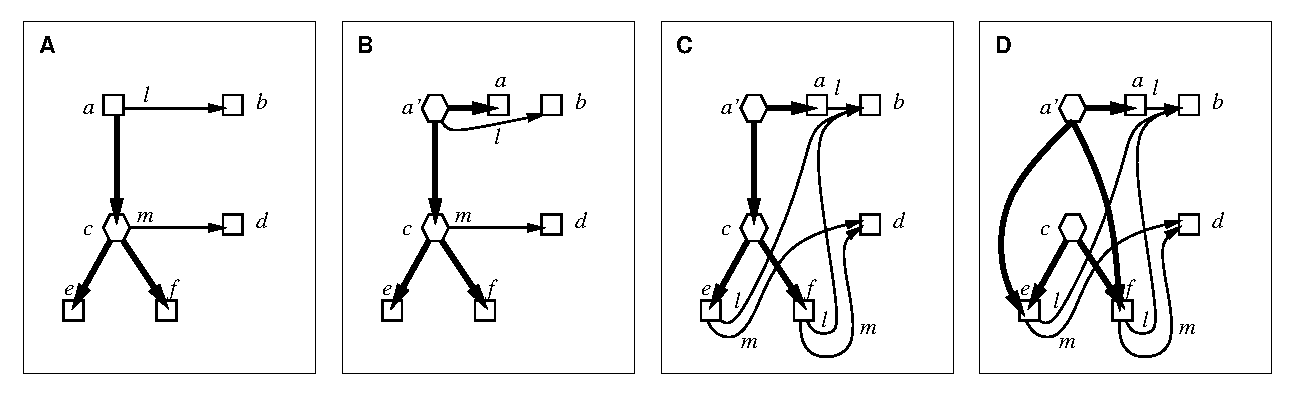
\psfig{file=simplify.ps,width=6.5in}}
\caption{\em
An example of class graph simplification. {\sf A}: the original class
graph.  Concrete classes are depicted as squares, and abstract classes
are hexagons.  Reference edges are regular, and subclass edges are
heavy.  {\sf B}: after step \protect\ref{step-introduce}.  {\sf C}:
after step \protect\ref{step-simpleten}.  {\sf D}: after step
\protect\ref{step-contract}.  }
\label{fig-simplify}
\end{figure}
\begin{enumerate}
\item
\label{step-introduce}
For each concrete class $v\in V$ with an outgoing subclass edge $\edge
v\diamond u\in E$, add a new abstract node $v'$ into $V$, along with
the following changes of the edge set:
\begin{itemize}
\item
Divert all edges coming into $v$ to end at $v'$. That is, 
$$
E\gets E\cup\Set{\edge u l v'\mid \edge u l v\in E}
 \setminus\Set{\edge u l v\mid  \edge u l v\in E}
$$
\item
Divert all subclass edges going out from $v$ to originate at $v'$. That is,
$$
E\gets E\cup\Set{\edge {v'} \diamond u\mid \edge v \diamond u\in E}
   \setminus\Set{\edge v \diamond u\mid \edge v \diamond u}
$$
\item
Make $v$ a subclass of $v'$:
$$E\gets E\cup\Set{\edge {v'}\diamond v}$$
\end{itemize}
When this step is completed, no concrete class has subclass edges going 
out from it.

\item
\label{step-simpleten}
For each concrete class $v$: add edges so that the set of edges going
out from $v$ is exactly the induced edges of $v$.  Then, delete all
reference edges going out from abstract classes.

\item
\label{step-contract}
Contract long inheritance chains.  For each abstract class $v$: find
all concrete classes $u$ which can be reached from $v$ using subclass
edges only, and add a subclass edge $\edge v\diamond u$ if one does
not exist already. Finally, delete all subclass edges leading to
abstract classes.
\end{enumerate}

Informally, Step~\ref{step-introduce} decouples the sub-classing role
from concrete classes by introducing an additional abstract class for
each class which has both subclass and reference edges going out from
it.

Step~\ref{step-simpleten} unfolds inherited reference edges by pushing
them down the subclass hierarchy.  This can be done efficiently by
traversing the subclass edges in a top-down fashion, starting with
nodes with no subclass edges coming into them, and ``collecting''
reference edges as we go down. Details are omitted.

Step~\ref{step-contract} can be viewed as taking the transitive
(non-reflexive) closure of the subclass relation. This step can be
done in parallel with Step~\ref{step-simpleten}.

For the bound on the size of the resulting graph, note first that only
Step~\ref{step-introduce} may change the number of nodes by at most
doubling it.  Next, note that since Steps~\ref{step-simpleten} and
\ref{step-contract} do not change the connectivity structure of the
graph, we can deal with each connected component separately. Consider
such a component with $n$ nodes. Since it is connected, there are at
least $n-1$ nodes in the component before Steps~\ref{step-simpleten}
and~\ref{step-contract}.  Since these steps do not introduce nodes or
parallel edges, they may introduce at most $O(n^2)$ new edges.  We may
therefore conclude that the number of nodes in $\Simple(G)$ is at most
doubled and the number of edges is at most squared.


\section{Target language for static compilation}
\label{sec-target}
%%%%%%%%%%%%%%%%%%%%%%%%%%%%%%%%
Static traversal compilers compile strategies and class graphs into an
object-oriented program where the sequence of methods invoked by an
object depends only on the object structure and the method name (no
parameter passing is allowed).  Formally, the language is defined as
follows.

A {\em program} in the target language is a partial function which
maps a class name and a method name to a method.  A method is a tuple
of the form $\interval{l_1.m_1,\ldots, l_n.m_n}$, where $l_1\ldots l_n
\in\cL$ and $m_1\ldots m_n$ are method names.  When invoked, such a
method executes by invoking $l_i.m_i$ in order.  We distinguish two
kinds of methods: {\em visiting} and {\em non-visiting}, prescribed by
a predicate $\Visit$ defined on the set of method names.

An invocation of a program is defined as follows.  If $\Omega$ is an
object graph, $o$ a node in $\Omega$, $m$ a method name, $\Prog$ a
program in the target language, and $H$ a sequence of objects, then
the judgment
\[
\Omega \vdash_c o:m:\Prog \rhd H
\]
means that when sending the message $m$ to $o$, we get a traversal of
the object graph $\Omega$ starting in $o$ so that $H$ is the traversal
history.  Formally, this holds when the judgment is derivable using
the following rules:
\[
\hspace*{1.5cm}
\irule{\Omega \vdash_c o_i:m_i: \Prog \rhd H_i \air \forall i \in 1..n}
      {\Omega \vdash_c o:m: \Prog \rhd o \cdot H_1  \cdot ... \cdot H_n} 
   ~~~~~~
      \parbox{3in}{
       if $\Prog(\Class(o),m) = \interval{l_1.m_1\ldots l_n.m_n}$, and \\
          $\Visit(m)$,
         and $\edge o {l_i} {o_i} \mbox{ is in } \Omega
                \mbox{ for all }     i \in 1..n$.}
\]
and 
\[
\hspace*{1.5cm}
\irule{\Omega \vdash_c o_i:m_i: \Prog \rhd H_i \air \forall i \in 1..n}
      {\Omega \vdash_c o:m: \Prog \rhd  H_1  \cdot ... \cdot H_n} 
   ~~~~~~
      \parbox{3in}{
       if $\Prog(\Class(o),m) = \interval{l_1.m_1\ldots l_n.m_n}$, and \\
          $\neg\Visit(m)$, and $\edge o {l_i} {o_i} \mbox{ is in } \Omega 
                  \mbox{ for all } i \in 1..n$.}
\]
The label $c$ of the turnstile indicates ``code''.  Intuitively, the
rule says that when sending the message $m$ to $o$, we check if $o$
understands the message, and if so, we invoke the method. The object
$o$ is added to the traversal history only if $\Visit(m)$ is true.
Notice that for $n=0$, the rule is an axiom; in the case that
$\Visit(m)$ is true, it is simply
\[
\hspace*{3.5cm} 
\irule{}
      {\Omega \vdash_c o:m: \Prog \rhd o }
   ~~~~~~
      \parbox{3in}{
       if $\Prog(\Class(o),m) = \interval{}$}
\]
and if $\Visit(m)$ is false, then it is
\[
\hspace*{3.5cm}
\irule{}
      {\Omega \vdash_c o:m: \Prog \rhd \epsilon }
   ~~~~~~
      \parbox{3in}{
       if $\Prog(\Class(o),m) = \interval{}$,}
\]
where $\epsilon$ denotes the empty history.

Given a program in the target language, it is straightforward to
generate, for example, a \C++ or a Java program.

\end{document}
